\documentclass{article}

\usepackage{etoolbox}

% Set this toggle true to compile a version for the arxiv, and
% false to compile for the currently configured conference.
% NOTE: you also must set the single_column flags in the Rnw files to
% make side-by-side figures for the arxiv version.
\newtoggle{for_arxiv}
%\toggletrue{for_arxiv}
\togglefalse{for_arxiv}

\nottoggle{for_arxiv}{%
    \usepackage[accepted]{aistats2019} % hooray!
    % \usepackage{aistats2019}
}

\usepackage{microtype}
\usepackage{graphicx}
\usepackage{subfigure}
\usepackage{booktabs} % for professional tables
\usepackage{siunitx}
\usepackage{hyperref}
\usepackage{xargs}[2008/03/08]

\iftoggle{for_arxiv} {
    \usepackage[authoryear]{natbib}
} {
    \usepackage[round]{natbib}
    \renewcommand{\bibname}{References}
    \renewcommand{\bibsection}{\subsubsection*{\bibname}}
}


% Attempt to make hyperref and algorithmic work together better:
\newcommand{\theHalgorithm}{\arabic{algorithm}}


\usepackage{prettyref}
\usepackage{refstyle}

\usepackage{amsmath}
\usepackage{amssymb}
\usepackage{amsfonts}
\usepackage{amsthm}
\usepackage{mathrsfs}
\usepackage{mathtools}
\usepackage{colonequals}
\usepackage{algpseudocode, algorithm} %typical alg typesetting packages

\usepackage{listings}
\usepackage{pdfpages}

% Define things needed to incorporate the LyX appendix.
% We can define things redundantly if necessary, but please don't modify
% this file -- if there's a name clash for a function you want to define,
% please just pick a new name.

%%%%%%%%%%%%%%%%%%%%%%%
% BEGIN LYX STUFF

% Please don't edit this section manually. It's fussy and hard to get it to work.
% As it currently is, we can incorporate files from LyX.

% Please copy these from LyX so we can use both styles of writing
\AtBeginDocument{\providecommand\assuref[1]{\ref{assu:#1}}}
\AtBeginDocument{\providecommand\condref[1]{\ref{cond:#1}}}
\AtBeginDocument{\providecommand\lemref[1]{\ref{lem:#1}}}
\AtBeginDocument{\providecommand\defrefref[1]{\ref{defref:#1}}}
\AtBeginDocument{\providecommand\proprefref[1]{\ref{propref:#1}}}
\AtBeginDocument{\providecommand\thmrefref[1]{\ref{thmref:#1}}}
\AtBeginDocument{\providecommand\corref[1]{\ref{corref:#1}}}

\theoremstyle{plain}
    \ifx\thechapter\undefined
      \newtheorem{assumption}{\protect\assumptionname}
    \else
      \newtheorem{assumption}{\protect\assumptionname}[chapter]
    \fi
\theoremstyle{definition}
    \ifx\thechapter\undefined
      \newtheorem{defn}{\protect\definitionname}
    \else
      \newtheorem{defn}{\protect\definitionname}[chapter]
    \fi
\theoremstyle{plain}
    \ifx\thechapter\undefined
      \newtheorem{condition}{\protect\conditionname}
    \else
      \newtheorem{condition}{\protect\conditionname}[chapter]
    \fi
\theoremstyle{plain}
    \ifx\thechapter\undefined
      \newtheorem{prop}{\protect\propositionname}
    \else
      \newtheorem{prop}{\protect\propositionname}[chapter]
    \fi
\theoremstyle{plain}
    \ifx\thechapter\undefined
      \newtheorem{lem}{\protect\lemmaname}
    \else
      \newtheorem{lem}{\protect\lemmaname}[chapter]
    \fi
\theoremstyle{plain}
    \ifx\thechapter\undefined
	    \newtheorem{thm}{\protect\theoremname}
	  \else
      \newtheorem{thm}{\protect\theoremname}[chapter]
    \fi
\theoremstyle{plain}
    \ifx\thechapter\undefined
  \newtheorem{cor}{\protect\corollaryname}
\else
      \newtheorem{cor}{\protect\corollaryname}[chapter]
    \fi

%%%%%%%%%%%%%%%%%%%%%%%%%%%%%% User specified LaTeX commands.
\newref{cond}{refcmd={Condition \ref{#1}}}
\newref{assu}{refcmd={Assumption \ref{#1}}}
\newref{propref}{refcmd={Proposition \ref{#1}}}
\newref{corref}{refcmd={Corrolary \ref{#1}}}
\newref{lem}{refcmd={Lemma \ref{#1}}}
\newref{defref}{refcmd={Definition \ref{#1}}}
\newref{thmref}{refcmd={Theorem \ref{#1}}}

\makeatother

%\usepackage{babel}
\providecommand{\assumptionname}{Assumption}
\providecommand{\conditionname}{Condition}
\providecommand{\corollaryname}{Corollary}
\providecommand{\definitionname}{Definition}
\providecommand{\lemmaname}{Lemma}
\providecommand{\propositionname}{Proposition}
\providecommand{\theoremname}{Theorem}

\global\long\def\at#1{\rvert_{#1}}

\global\long\def\norm#1{\left\Vert #1\right\Vert }

\global\long\def\mbe{\mathbb{E}}

\global\long\def\thetahat{\hat{\theta}}

\global\long\def\onevec{1_{w}}

\global\long\def\thetawiggle{\tilde{\theta}}

\global\long\def\thetaone{\hat{\theta}_{1}}

\global\long\def\thetaij{\hat{\theta}_{\textrm{IJ}}}

\newcommandx\thetaw[1][usedefault, addprefix=\global, 1=w]{\hat{\theta}\left(#1\right)}

\global\long\def\hone{H_{1}}

\global\long\def\constij{C_{\textrm{IJ}}}

\global\long\def\consth{C_{h}}

\global\long\def\constg{C_{g}}

\global\long\def\constw{C_{w}}

\newcommandx\constop[1][usedefault, addprefix=\global, 1={\text{\,}}]{C_{op}^{#1}}

\global\long\def\liph{L_{h}}

\global\long\def\thetasize{\Delta_{\theta}}

\global\long\def\deltasize{\Delta_{\delta}}

\global\long\def\thetaball{B_{\Delta_{\theta}}}

\global\long\def\thetadeltaball{B_{C_{op}\delta}}


% END LYX STUFF
%%%%%%%%%%%%%%%%%%%%%%%


% This picks up the knitr boilerplate, allowing us to \input partial knitr
% documents.
\usepackage[]{graphicx}
\usepackage[]{color}
%% maxwidth is the original width if it is less than linewidth
%% otherwise use linewidth (to make sure the graphics do not exceed the margin)
\makeatletter
\def\maxwidth{ %
  \ifdim\Gin@nat@width>\linewidth
    \linewidth
  \else
    \Gin@nat@width
  \fi
}
\makeatother

\definecolor{fgcolor}{rgb}{0.345, 0.345, 0.345}
\newcommand{\hlnum}[1]{\textcolor[rgb]{0.686,0.059,0.569}{#1}}%
\newcommand{\hlstr}[1]{\textcolor[rgb]{0.192,0.494,0.8}{#1}}%
\newcommand{\hlcom}[1]{\textcolor[rgb]{0.678,0.584,0.686}{\textit{#1}}}%
\newcommand{\hlopt}[1]{\textcolor[rgb]{0,0,0}{#1}}%
\newcommand{\hlstd}[1]{\textcolor[rgb]{0.345,0.345,0.345}{#1}}%
\newcommand{\hlkwa}[1]{\textcolor[rgb]{0.161,0.373,0.58}{\textbf{#1}}}%
\newcommand{\hlkwb}[1]{\textcolor[rgb]{0.69,0.353,0.396}{#1}}%
\newcommand{\hlkwc}[1]{\textcolor[rgb]{0.333,0.667,0.333}{#1}}%
\newcommand{\hlkwd}[1]{\textcolor[rgb]{0.737,0.353,0.396}{\textbf{#1}}}%
\let\hlipl\hlkwb

\usepackage{framed}
\makeatletter
\newenvironment{kframe}{%
 \def\at@end@of@kframe{}%
 \ifinner\ifhmode%
  \def\at@end@of@kframe{\end{minipage}}%
  \begin{minipage}{\columnwidth}%
 \fi\fi%
 \def\FrameCommand##1{\hskip\@totalleftmargin \hskip-\fboxsep
 \colorbox{shadecolor}{##1}\hskip-\fboxsep
     % There is no \\@totalrightmargin, so:
     \hskip-\linewidth \hskip-\@totalleftmargin \hskip\columnwidth}%
 \MakeFramed {\advance\hsize-\width
   \@totalleftmargin\z@ \linewidth\hsize
   \@setminipage}}%
 {\par\unskip\endMakeFramed%
 \at@end@of@kframe}
\makeatother

\definecolor{shadecolor}{rgb}{.97, .97, .97}
\definecolor{messagecolor}{rgb}{0, 0, 0}
\definecolor{warningcolor}{rgb}{1, 0, 1}
\definecolor{errorcolor}{rgb}{1, 0, 0}
\newenvironment{knitrout}{}{} % an empty environment to be redefined in TeX

\usepackage{alltt}


% Paper-specific math macros (not in the appendix).
\global\long\def\wcv{W_k}
\global\long\def\wboot{W^*_B}
\global\long\def\thetapw{\thetahat(w)}
\global\long\def\wdiff{\Delta w}


\newcommand{\eq}[1]{Eq.~\ref{eq:#1}}
\newcommand{\fig}[1]{Fig.~\ref{fig:#1}}
\newcommand{\rthm}[1]{Theorem~\ref{thm:#1}}
\newcommand{\sect}[1]{Section~\ref{sec:#1}}
\newcommand{\subsect}[1]{Section~\ref{subsec:#1}}
\newcommand{\assum}[1]{Assumption~\ref{assum:#1}}
\newcommand{\lemma}[1]{Lemma~\ref{lm:#1}}
\newcommand{\corollary}[1]{Corollary~\ref{cor:#1}}
\newcommand{\app}[1]{Appendix~\ref{app:#1}}
\newcommand{\appsect}[1]{Appendix~\ref{sec:#1}}

\newcommand{\coreassum}{Assumptions \ref{assu:paper_smoothness}--\ref{assu:paper_lipschitz} }
\newcommand{\paperallcoreassum}{Assumptions \ref{assu:paper_smoothness}--\ref{assu:paper_weight_bounded} }

\iftoggle{for_arxiv}{%
    \title{A Swiss Army Infinitesimal Jackknife}
    \author{
      Ryan Giordano\\ \texttt{rgiordano@berkeley.edu}
      \and
      Will Stephenson\\ \texttt{wtstephe@mit.edu}
      \and
      Runjing Liu\\ \texttt{runjing\_liu@berkeley.edu}
      \and
      Michael I.~Jordan\\ \texttt{jordan@cs.berkeley.edu}
      \and
      Tamara Broderick\\ \texttt{tbroderick@csail.mit.edu}
    }
}


\begin{document}

\iftoggle{for_arxiv} {
    \maketitle
}

\nottoggle{for_arxiv} {
\twocolumn[
    \aistatstitle{A Swiss Army Infinitesimal Jackknife}

    \aistatsauthor{
        Ryan Giordano \And
        Will Stephenson \And
        Runjing Liu \And
        Michael I.~Jordan \And
        Tamara Broderick
    }
    \aistatsaddress{
        UC Berkeley \And
        MIT \And
        UC Berkeley \And
        UC Berkeley \And
        MIT
    }
]
}

\begin{abstract}
%
The error or variability of machine learning algorithms is often assessed by
repeatedly re-fitting a model with different weighted versions of the observed
data. The ubiquitous tools of cross-validation (CV) and the bootstrap are
examples of this technique. These methods are powerful in large part due to
their model agnosticism but can be slow to run on modern, large data sets due to
the need to repeatedly re-fit the model. In this work, we use a linear
approximation to the dependence of the fitting procedure on the weights,
producing results that can be faster than repeated re-fitting by an order of
magnitude. This linear approximation is sometimes known as the ``infinitesimal
jackknife'' in the statistics literature, where it is mostly used as a
theoretical tool to prove asymptotic results. We provide explicit finite-sample
error bounds for the infinitesimal jackknife in terms of a small number of
simple, verifiable assumptions. Our results apply whether the weights and data
are stochastic or deterministic, and so can be used as a tool for proving the
accuracy of the infinitesimal jackknife on a wide variety of problems. As a
corollary, we state mild regularity conditions under which our approximation
consistently estimates true leave-$k$-out cross-validation for any fixed $k$.
These theoretical results, together with modern automatic differentiation
software, support the application of the infinitesimal jackknife to a wide
variety of practical problems in machine learning, providing a ``Swiss Army
infinitesimal jackknife.'' We demonstrate the accuracy of our methods on a range
of simulated and real datasets.

%
\end{abstract}

\section{Introduction}\label{sec:introduction}

Statistical machine learning methods are increasingly deployed in real-world
problem domains where they are the basis of decisions affecting individuals'
employment, savings, health, and safety. Unavoidable randomness in data
collection necessitates understanding how our estimates, and resulting
decisions, might have differed had we observed different data. Both cross
validation (CV) and the bootstrap attempt to diagnose this variation and are
widely used in classical data analysis. But these methods are often
prohibitively slow for modern, massive datasets, as they require running a
learning algorithm on many slightly different datasets.  In this work, we
propose to replace these many runs with a single perturbative approximation. We
show that the computation of this approximation is far cheaper than the
classical methods, and we provide theoretical conditions that establish its
accuracy.

Many data analyses proceed by minimizing a loss function of exchangeable data.
Examples include empirical loss minimization and M-estimation based on product
likelihoods. Since we typically do not know the true distribution generating the
data, it is common to approximate the dependence of our estimator on the data
via the dependence of the estimator on the empirical distribution. In
particular, we often form a new, proxy dataset using random or deterministic
modifications of the empirical distribution, such as randomly removing $k$
datapoints for leave-$k$-out CV. A proxy dataset obtained in this way can be
represented as a weighting of the original data. From a set of such proxy
datasets we can obtain estimates of uncertainty, including estimates of bias,
variance, and prediction accuracy.

As data and models grow, the cost of repeatedly solving a large optimization
problem for a number of different values of weights can become impractically
large. Conversely, though, larger datasets often exhibit greater regularity; in
particular, under fairly general conditions, limit laws based on independence
imply that an optimum exhibits diminishing dependence on any fixed set of data
points.  We use this observation to derive a linear approximation to resampling
that needs to be calculated only once, but which nonetheless captures the
variability inherent in the repeated computations of classical CV.  Our method
is an instance of the \emph{infinitesimal jackknife} (IJ), a general methodology
that was historically a precursor to cross-validation and the
bootstrap~\citep{jaeckel:1972:infinitesimal, efron:1982:jackknife}. Part of our
argument is that variants of the IJ should be reconsidered
for modern large-scale applications because, for smooth optimization problems,
the IJ can be calculated automatically with modern
automatic differentiation tools \citep{baydin:2015:automatic}.

By using this linear approximation, we incur the cost of forming and inverting a
matrix of second derivatives with size equal to the dimension of the parameter
space, but we avoid the cost of repeatedly re-optimizing the objective. As we
demonstrate empirically, this tradeoff can be extremely favorable in many
problems of interest.

Our approach aims to provide a felicitous union of two schools of thought. In
statistics, the IJ is typically used to prove normality or
consistency of other estimators~\citep{
fernholz:1983:mises,shao:1993:jackknifemestimator,shao:2012:jackknife}. However,
the conditions that are required for these asymptotic analyses to hold are
prohibitively restrictive for machine learning---specifically, they require
objectives with bounded gradients. A number of recent papers in machine learning
have provided related linear approximations for the special case of
leave-one-out cross-validation~\citep{KohL17, RadM18, BeiramiRST17}, though
their analyses lack the generality of the statistical perspective.

We combine these two approaches by modifying the proof of the Fr{\'e}chet
differentiability of M-estimators developed by \citet{clarke:1983:uniqueness}.
Specifically, we adapt the proof away from the question of Fr{\'e}chet
differentiability within the class of all empirical distributions to the
narrower problem of approximating the exact re-weighting on a particular dataset
with a potentially restricted set of weights.  This limitation of what we expect
from the approximation is crucial; it allows us to bound the error in terms of a
complexity measure of the set of derivatives of the observed objective function,
providing a basis for non-asymptotic applications in large-scale machine
learning, even for objectives with unbounded derivatives.  Together with modern
automatic differentiation tools, these results extend the use of the
IJ to a wider range of practical problems. Thus, our
``Swiss Army infinitesimal jackknife,'' like the famous Swiss Army knife, is a
single tool with many different functions.



\section{Methods and Results}\label{sec:methods}

\subsection{Problem definition}\label{subsec:problem_definition}
We consider the problem of estimating an unknown parameter
$\theta\in\Omega_{\theta}\subseteq\mathbb{R}^{D}$, with a compact
$\Omega_{\theta}$ and a dataset of size $N$. Our analysis will proceed entirely
in terms of a fixed dataset, though we will be careful to make assumptions that
will plausibly hold for all $N$ under suitably well-behaved random sampling. We
define our estimate, $\thetahat\in\Omega_{\theta}$, as the root of a weighted
estimating equation. For each $n=1, \ldots, N$, let $g_{n}\left(\theta\right)$ be a
function from $\Omega_{\theta}$ to $\mathbb{R}^{D}$. Let $w_{n}$ be a real
number, and let $w$ be the vector collecting the $w_n$.
Then $\thetahat$ is defined as the quantity that satisfies
%
\begin{align}
\thetapw:= &
    \quad\theta\textrm{ such that }
    \frac{1}{N}\sum_{n=1}^{N}w_{n}g_{n}\left(\theta\right) = 0.
    \label{eq:estimating_equation}
\end{align}
%
We will impose assumptions below that imply at least local uniqueness of
$\thetapw$; see the discussion following \assuref{paper_hessian} in
\subsect{assumptions}.

As an example, consider a family of continuously differentiable loss functions
$f\left(\cdot, \theta\right)$ parameterized by $\theta$ and evaluated at data
points $x_{n},n=1, \ldots, N$. If we want to solve the optimization problem
%
$\thetahat=\underset{\theta\in\Omega_{\theta}}
    {\mathrm{argmin}}\frac{1}{N}\sum_{n=1}^{N}f\left(x_{n},\theta\right),$
%
then we take $g_{n}\left(\theta\right)=\partial
f\left(x_{n},\theta\right)/\partial\theta$ and $w_{n}\equiv1$. By keeping our
notation general, we will be able to analyze a more general class of problems,
such as multi-stage optimization (see \sect{genomics}). However, to aid
intuition, we will sometimes refer to the $g_{n}\left(\theta\right)$ as
``gradients'' and their derivatives as ``Hessians.''

When \eqref{estimating_equation} is not degenerate (we articulate precise
conditions below), $\thetahat$ is a function of the weights through solving the
estimating equation, and we write $\thetapw$ to emphasize this.
We will focus on the case where we have solved \eqref{estimating_equation} for
the weight vector of all ones, $\onevec:=\left(1, \ldots, 1\right)$, which we denote
$\thetaone := \thetahat\left(\onevec\right)$.

A re-sampling scheme can be specified by choosing a set
$W\subseteq\mathbb{R}^{N}$ of weight vectors. For example, to approximate
leave-$k$-out CV, one repeatedly computes $\thetapw$ where $w$ has $k$ randomly
chosen zeros and all ones otherwise.  Define $\wcv$ as the set of every possible
leave-$k$-out weight vector.  Showing that our approximation is good for all
leave-$k$-out analyses with probability one is equivalent to showing that the
approximation is good for all $w \in \wcv$.

In the case of the bootstrap, $W$ contains a fixed number $B$ of randomly chosen
weight vectors,
$w_{b}^{*}\stackrel{iid}{\sim}\mathrm{Multinomial}\left(N,N^{-1}\right)$ for
$b=1, \ldots, B$, so that $\sum_{n=1}^N w_{bn}^{*} = N$ for each $b$. Note that
while $w_n$ or $w_{bn}^{*}$ are scalars, $w_{b}^{*}$ is a vector of length $N$.
The distribution of
$\thetahat\left(w_{b}^{*}\right)-\thetahat\left(\onevec\right)$ is then used to
estimate the sampling variation of $\thetaone$. Define this set $\wboot =
\{w_{1}^{*},\ldots,w_{B}^{*}\}$.  Note that $\wboot$ is stochastic and is a
subset of all weight vectors that sum to $N$.

In general, $W$ can be deterministic or stochastic, may contain integer or
non-integer values, and may be determined independently of the data or jointly
with it. As with the data, our results hold for a given $W$, but in a way that
will allow natural high-probability extensions to stochastic $W$.


\subsection{Linear approximation}

The main problem we solve is the computational expense involved in evaluating
$\thetapw$ for all the $w\in W$. Our contribution is to use only quantities
calculated from $\thetaone$ to approximate $\thetapw$ for all $w\in W$, without
re-solving \eqref{estimating_equation}. Our approximation is based on the
derivative $\frac{d\thetapw}{dw^{T}}$, whose existence depends on the
derivatives of $g_{n}\left(\theta\right)$, which we assume to exist, and which
we denote as $h_{n}\left(\theta\right):=\frac{\partial
g_{n}\left(\theta\right)}{\partial\theta^{T}}$. We use this notation because
$h_{n}\left(\theta\right)$ would be the Hessian of a term of the objective in
the case of an optimization problem. We make the following definition for
brevity.
%
\begin{defn}
The fixed point equation and its derivative are given respectively by
%
\begin{align*}
G\left(\theta,w\right) &:=
    \frac{1}{N}\sum_{n=1}^{N}w_{n}g_{n}\left(\theta\right) \\
H\left(\theta,w\right) &:=
    \frac{1}{N}\sum_{n=1}^{N}w_{n}h_{n}\left(\theta\right).
\end{align*}
%
\end{defn}
%
Note that $G\left(\thetapw,w\right)=0$ because $\thetapw$ solves
\eqref{estimating_equation} for $w$. We define
$\hone:=H\left(\thetaone,\onevec\right)$ and define the weight difference as
$\wdiff=w-\onevec\in\mathbb{R}^{N}$. When $\hone$ is invertible, one can use the
implicit function theorem and the chain rule to show that the derivative of
$\thetapw$ with respect to $w$ is given by
%
\begin{align*}
\frac{d\thetapw}{dw^{T}}\at{\onevec}\wdiff & =
    -\hone^{-1}\frac{1}{N}\sum_{n=1}^{N}g_{n}
    \left(\thetaone\right)\wdiff \\
    & =-\hone^{-1}G\left(\thetaone,\wdiff\right).
\end{align*}
%
This derivative allows us to form a first-order approximation to $\thetapw$
at $\thetaone$.
%
\begin{defn}
\label{defref:ij_definition}Our linear approximation to $\thetapw$
is given by
%
\begin{align*}
\thetaij\left(w\right) & :=\thetaone-\hone^{-1}G\left(\thetaone,\wdiff\right).
\end{align*}
\end{defn}
%
We use the subscript ``IJ'' for ``infinitesimal jackknife,'' which is the name
for this estimate in the statistics literature
\citep{jaeckel:1972:infinitesimal,shao:1993:jackknifemestimator}. Because
$\thetaij$ depends only on $\thetaone$ and $\wdiff$, and not on
solutions at any other values of $w$, there is no
need to re-solve \eqref{estimating_equation}. Instead, to calculate $\thetaij$
one must solve a linear system involving $\hone$. Recalling that $\theta$ is
$D$-dimensional, the calculation of $\hone^{-1}$ (or a factorization that
supports efficient solution of linear systems) can be $O\left(D^{3}\right)$.
However, once $\hone^{-1}$ is calculated or $\hone$ is factorized, calculating our approximation
$\thetaij\left(w\right)$ for each new weight costs only as
much as a single matrix-vector multiplication. Furthermore, $\hone$ often has a
sparse structure allowing $\hone^{-1}$ to be calculated more efficiently than a
worst-case scenario (see \sect{genomics} for an example). In more
high-dimensional examples with dense Hessian matrices, such as neural networks,
one may need to turn to approximations such as stochastic second-order methods
\citep{KohL17, agarwal:2016:lissa} and conjugate gradient
\citep{wright:1999:optimization}. Indeed, even in relatively small or sparse
problems, the vast bulk of the computation required to calculate $\thetaij$ is
in the computation of $\hone^{-1}$. We leave the important question of
approximate calculation of $\hone^{-1}$ for future work.


\subsection{Assumptions and results}\label{subsec:assumptions}

We now state our key assumptions and results, which are sufficient conditions
under which $\thetaij(w)$ will be a good approximation to $\thetapw$. We defer
most proofs to \appsect{appendix_proofs}. We use $\norm{\cdot}_{op}$
to denote the matrix operator norm, $\norm{\cdot}_{2}$ to denote the $L_{2}$
norm, and $\norm{\cdot}_{1}$ to denote the $L_{1}$ norm. For quantities like $g$
and $h$, which have dimensions $N\times D$ and $N\times D\times D$ respectively,
we apply the $L_p$ norm to the vectorized version of arrays.
%
For example,
$\frac{1}{\sqrt{N}} \norm{h\left(\theta\right)}_{2} =
\sqrt{
\frac{1}{N}\sum_{n=1}^{N}\sum_{i=1}^{D}\sum_{j=1}^{D}
\left[h_{n}\left(\theta\right)\right]_{ij}^{2}
}$ which is the square root of a sample average over $n\in[N]$.

We state all assumptions and results for a fixed $N$, a given estimating
equation vector $g\left(\theta\right)$, and a fixed class of weights $W$.
Although our analysis proceeds
with these quantities fixed, we are careful to make only assumptions that can
plausibly hold for all $N$ and/or for randomly chosen $W$
under appropriate regularity conditions.
%
\begin{assumption}[Smoothness] \label{assu:paper_smoothness}
For all $\theta\in\Omega_{\theta}$, each $g_{n}\left(\theta\right)$
is continuously differentiable in $\theta$.
\end{assumption}
%
The smoothness in \assuref{paper_smoothness} is necessary
for a local approximation like \defrefref{ij_definition} to have
any hope of being useful.
%
\begin{assumption}[Non-degeneracy]
\label{assu:paper_hessian}
For all $\theta\in\Omega_{\theta}$, $H\left(\theta,\onevec\right)$
is non-singular, with
$\sup_{\theta\in\Omega_{\theta}}\norm{H\left(\theta,\onevec\right)^{-1}}_{op}
\le\constop < \infty$.
\end{assumption}
%
Without \assuref{paper_hessian}, the derivative in \defrefref{ij_definition}
would not exist. For an optimization problem, \defrefref{ij_definition} amounts
to assuming that the Hessian is strongly positive definite, and, in general,
assures that the solution $\thetaone$ is unique.  Under our assumptions, we will
show later that, additionally, $\thetapw$ is unique in a neighborhood of
$\thetaone$; see \lemref{continuous_invertibility} of \appsect{appendix_proofs}.
Furthermore, by fixing $\constop$, if we want to apply \assuref{paper_hessian}
for $N\rightarrow\infty$, we will require that $\hone$ remains strongly positive
definite.

%
\begin{assumption}[Bounded averages] \label{assu:paper_bounded}
There exist finite constants $\constg$ and $\consth$ such that
$\sup_{\theta\in\Omega_{\theta}}
    \frac{1}{\sqrt{N}} \norm{g\left(\theta\right)}_{2}\le\constg<\infty
\quad\textrm{and}\quad
\sup_{\theta\in\Omega_{\theta}}
    \frac{1}{\sqrt{N}} \norm{h\left(\theta\right)}_{2} \le\consth<\infty$.
\end{assumption}
%
\assuref{paper_bounded} essentially states that the sample variances of the
gradients and Hessians are uniformly bounded. Note that it does not require that
these quantities are bounded term-wise. For example, we allow
$\sup_{n}\norm{g_{n}\left(\theta\right)}_2^2
\underset{N\rightarrow\infty}{\longrightarrow}\infty$, as long as
$\sup_{n}\frac{1}{N}\norm{g_{n}\left(\theta\right)}^{2}_2$ remains bounded. This
is a key advantage of the present work over many past applications of the IJ to
M-estimation, which require $\sup_n \norm{g_n(\theta)}_2^2$ to be uniformly
bounded for all $N$ \citep{shao:2012:jackknife, BeiramiRST17}.

In both machine learning and
statistics, $\sup_n\norm{g_n(\theta)}_2^2$ is rarely bounded, though
$\frac{1}{N}\norm{g(\theta)}_2^2$ often is.  As a simple example, suppose
that $\theta \in \mathbb{R}^1$, $x_n \sim \mathcal{N}(0, 1)$, and
$g_n = \theta - x_n$, as would arise from the squared error loss
$f_n\left(x_n, \theta\right) = \frac{1}{2}\left(\theta - x_n\right)^2$.
Fix a $\theta$ and let $N \rightarrow \infty$.  Then
$\sup_n\norm{g_n(\theta)}_2^2 \rightarrow \infty$ because
$\sup_n |x_n| \rightarrow \infty$, but
$\frac{1}{N}\norm{g(\theta)}_2^2 \rightarrow \theta^2 + 1$ by the law of
large numbers.
%
\begin{assumption}[Local smoothness] \label{assu:paper_lipschitz}
There exists a $\thetasize>0$ and a finite constant $\liph$ such that,
$\norm{\theta-\thetaone}_{2} \le \thetasize$ implies that
$\frac{\norm{h\left(\theta\right)-h\left(\thetaone\right)}_{2}}
    {\sqrt{N}}\le\liph\norm{\theta-\thetaone}_{2}$.
\end{assumption}
%
The constants defined in \assuref{paper_lipschitz} are needed to calculate
our error bounds explicitly.

\coreassum are quite general and should be expected to hold for many reasonable
problems, including holding uniformly asymptotically with high probability for
many reasonable data-generating distributions, as the following lemma shows.
%
\begin{lem}[The assumptions hold under uniform convergence]
\label{lem:assumptions_hold}
%
Let $\Omega_{\theta}$ be a compact set, and let
$g_{n}\left(\theta\right)$ be twice continuously differentiable IID random
functions for $n \in [N]$.  (The function is random but $\theta$ is not---for example,
$\mbe\left[g_n(\theta)\right]$ is still a function of $\theta$.)
Define
$r_{n}\left(\theta\right) :=
    \frac{\partial^{2}g{}_{n}\left(\theta\right)}
    {\partial\theta\partial\theta}$,
so $r_{n}\left(\theta\right)$ is a $D\times D\times D$ tensor.

Assume that we can exchange integration and differentiation, that
$\mbe\left[h_{n}\left(\theta\right)\right]$ is non-singular for
all $\theta\in\Omega_{\theta}$,
and that all of
$\mbe\left[\sup_{\theta\in\Omega_{\theta}}\norm{g_{n}\left(\theta\right)}_{2}^{2}\right]$,
$\mbe\left[\sup_{\theta\in\Omega_{\theta}}\norm{h_{n}\left(\theta\right)}_{2}^{2}\right]$,
and
$\mbe\left[\sup_{\theta\in\Omega_{\theta}}\norm{r_{n}\left(\theta\right)}_{2}^{2}\right]$
are finite.

Then $\lim_{N\rightarrow\infty}P\left(\textrm{\coreassum\ hold}\right)=1$.
%
\end{lem}
%
\lemref{assumptions_hold} follows from
the uniform convergence results of Theorems 9.1 and 9.2 in
\citet{keener:2011:theoretical}.
See \appsect{use_cases} for a detailed proof.  A common example to which
\lemref{assumptions_hold} would apply is where $x_n$ are well-behaved
IID data and $g_n(\theta) = \gamma(x_n, \theta)$ for an appropriately
smooth estimating function $\gamma(\cdot, \theta)$.
See \citet[Chapter 9]{keener:2011:theoretical} for more details and examples,
including applications to maximum likelihood estimators on unbounded domains.

\coreassum apply to the estimating equation.  We also require
a boundedness condition for $W$.
%
\begin{assumption}[Bounded weight averages] \label{assu:paper_weight_bounded}
The quantity
$\frac{1}{\sqrt{N}}\norm w_{2}$ is uniformly bounded for $w\in W$ by a finite
constant $\constw$.
\end{assumption}
%
Our final requirement is considerably more restrictive, and
contains the essence of whether or not $\thetaij(w)$ will be a good approximation
to $\thetapw$.
%
\begin{condition}[Set complexity]
    %
\label{cond:paper_uniform_bound}There exists a $\delta\ge0$ and
a corresponding set $W_{\delta}\subseteq W$ such that
%
\begin{align*}
\sup_{w\in W_{\delta}}\sup_{
    \theta\in\Omega_{\theta}} &\norm{\frac{1}{N}\sum_{n=1}^{N}
    \left(w_{n}-1\right)g_{n}\left(\theta\right)}_{1}  \le\delta
\quad\textrm{and} \\
\sup_{w\in W_{\delta}}\sup_{
    \theta\in\Omega_{\theta}} &\norm{\frac{1}{N}\sum_{n=1}^{N}
    \left(w_{n}-1\right)h_{n}\left(\theta\right)}_{1}  \le\delta.
\end{align*}
\end{condition}
%
\condref{paper_uniform_bound} is central to establishing when the approximation
$\thetaij\left(w\right)$ is accurate. For a given $\delta$, $W_{\delta}$ will be
the class of weight vectors for which $\thetaij(w)$ is accurate to within order
$\delta$. Trivially, $\onevec\in W_{\delta}$ for $\delta=0$, so $W_{\delta}$ is
always non-empty, even for arbitrarily small $\delta$. The trick will be to
choose a small $\delta$ that still admits a large class $W_{\delta}$ of weight
vectors. In \sect{methods_examples} we will discuss
\condref{paper_uniform_bound} in more depth, but it will help to first state our
main theorem.
%
\begin{defn}
\label{defref:constants_definition}  The following constants are given by
quantities in \paperallcoreassum.
\begin{align*}
    \constij &:= 1+D \constw \liph \constop \\
    \deltasize &:=
        \min\left\{ \thetasize\constop[-1],
                    \frac{1}{2}\constij^{-1}\constop[-1]\right\}.
\end{align*}
\end{defn}
%
Note that, although the parameter dimension $D$ occurs explicitly only once in
\defrefref{constants_definition}, all of $\constw$, $\constop$, and $\liph$ in
general might also contain dimension dependence. Additionally, the bound
$\delta$ in \condref{paper_uniform_bound}, a measure of the set complexity of
the parameters, will typically depend on dimension. However, the particular
place where the parameter dimension enters will depend on the problem and
asymptotic regime, and our goal is to provide an adaptable toolkit for a wide
variety of problems.

We are now ready to state our main result.
%
\begin{thm}[Error bound for the approximation]
\label{thmref:paper_ij_error}Under
\paperallcoreassum and \condref{paper_uniform_bound},
\begin{align*}
\delta\le \deltasize \Rightarrow
\max_{w\in W_{\delta}}\norm{\thetaij\left(w\right)-{\thetapw}}_{2}
    \le 2 \constop[2] \constij \delta^{2}.
\end{align*}
\end{thm}
%
We stress that \thmrefref{paper_ij_error} bounds only the difference between
$\thetaij(w)$ and $\thetapw$.  \thmrefref{paper_ij_error} alone does not
guarantee that $\thetaij(w)$ converges to any hypothetical infinite population
quantity. We see this as a strength, not a weakness.  To begin with, convergence
to an infinite population requires stronger assumptions.  Contrast, for example,
the Fr{\'e}chet differentiability work of \citet{clarke:1983:uniqueness}, on which
our work is based, with the stricter requirements in the proof of consistency in
\cite{shao:1993:jackknifemestimator}.  Second, machine learning problems may not
naturally admit a well-defined infinite population, and the dataset at hand may
be of primary interest. Finally, by  analyzing a particular sample rather than a
hypothetical infinite population, we can bound the error in terms of the
quantities $\constij$ and $\deltasize$, which can actually be calculated from the
data at hand.

Still, \thmrefref{paper_ij_error} is useful to prove asymptotic
results about the difference $\norm{\thetaij\left(w\right)-{\thetapw}}_{2}$.
As an illustration, we now show that the uniform consistency of leave-$k$-out
CV follows from \thmrefref{paper_ij_error} by a straightforward
application of H{\"o}lder's inequality.
%
\begin{cor}[Consistency for leave-$k$-out CV]
\label{cor:paper_k_means_consistent}
Assume that \paperallcoreassum hold uniformly for all $N$. Fix an integer
$k$, and let
%
$$
W_{k}:=\left\{ w:w_{n}=0\textrm{ in }k\textrm{ entries and }1\textrm{ otherwise}\right\} .
$$
%
Then, for all $N$, there exists a constant $C_K$ such that
\begin{align*}
\sup_{w\in W_{k}}\norm{\thetaij\left(w\right)-{\thetapw}}_{2}
    & \le C_K \frac{\norm g_{\infty}^2}{N^2} \\
    & \le C_K \frac{\max\left\{\constg, \consth\right\}^2}{N}.
\end{align*}
\end{cor}
%
\begin{proof}
For $w\in W_{k}$, $\frac{\norm{\wdiff}_{2}}{\sqrt{N}}=\sqrt{\frac{K}{N}}.$
Define $C_{gh} := \max\left\{\constg, \consth\right\}$.
By \assuref{paper_bounded},
$\norm g_{2}/\sqrt{N}\le C_{gh}$ and $\norm h_{2}/\sqrt{N}\le C_{gh}$
for all $N$. By H{\"o}lder's inequality,
\begin{align*}
\lefteqn{ \sup_{w\in W}\sup_{\theta\in\Omega_{\theta}}
    \norm{\frac{1}{N}\sum_{n=1}^{N}\left(w_{n}-1\right)g_{n}
        \left(\theta\right)}_{1} } \\
    & \le \sup_{w\in W} \norm{w - \onevec}_1
    	\sup_{\theta\in\Omega_{\theta}} \frac{\norm g_{\infty}}{N}
    =
    	K \frac{\norm g_{\infty}}{N} \le
    	K \frac{C_{gh}}{\sqrt{N}},
\end{align*}
with a similar bound for $\norm h_{2}$. Consequently, for $N$ large
enough, \condref{paper_uniform_bound} is satisfied with $W_{\delta}=W_{k}$
and either $\delta=K \frac{\norm g_{\infty}}{N}$
or $\delta=K \frac{C_{gh}}{\sqrt{N}}$.
The result then follows from \thmrefref{paper_ij_error}.
\end{proof}



\section{Examples}\label{sec:methods_examples}

The moral of \thmrefref{paper_ij_error} is that, under \paperallcoreassum and
\condref{paper_uniform_bound},
$\norm{\thetaij-{\thetaw}}=O\left(\delta^{2}\right)$ for $w\in W_{\delta}$. That
is, if we can make $\delta$ small enough, $W_{\delta}$ big enough, and still
satisfy \condref{paper_uniform_bound}, then $\thetaij\left(w\right)$ is a good
approximation to $\thetaw$ for ``most'' $w$, where ``most'' is defined as the size
of $W_\delta$. So it is worth taking a moment to develop some intuition for
\condref{paper_uniform_bound}. We have already seen in
\corollary{paper_k_means_consistent} that $\thetaij$ is, asymptotically, a good
approximation for leave-$k$-out CV uniformly in $W$. We now discuss some additional
cases: first, a worst-case example for which $\thetaij$ is not expected to work,
second the bootstrap, and finally we revisit leave-one-out cross
validation in the context of these other two methods.

First, consider a pathological example. Let $W_{full}$ be the set of all weight
vectors that sum to $N$. Let
$n^{*}=\max_{n\in[N]}\norm{g_{n}\left(\thetaone\right)}_{1}$ be the index of the
gradient term with the largest $L_{1}$ norm, and let $w_{n^{*}}=N$ and $w_n=0$
for $n \ne n^{*}$. Then
%
\begin{align*}
&\sup_{\theta\in\Omega_{\theta}}
    \norm{\frac{1}{N}\sum_{n=1}^{N}
        \left(w_{n}-1\right)g_{n}\left(\theta\right)}_{1} \\
&\quad =\sup_{\theta\in\Omega_{\theta}}
    \norm{g_{n^{*}}\left(\theta\right)-
        \frac{1}{N}\sum_{n=1}^{N}g_{n}\left(\theta\right)}_{1}
    \ge\norm{g_{n^{*}}\left(\thetaone\right)}_{1}.
\end{align*}
%
(The last inequality uses the fact that $G\left(\thetaone,\onevec\right)=0$.) In
this case, unless the largest gradient,
$\norm{g_{n^{*}}\left(\thetaone\right)}_{1}$, is small,
\condref{paper_uniform_bound} will not be satisfied for small $\delta$, and we
would not expect $\thetaij$ to be a good estimate for $\thetaw$ for all $w\in
W_{full}$. The class $W_{full}$ is too expressive. In the language of
\condref{paper_uniform_bound}, for some small fixed $\delta$, $W_{\delta}$ will
be some very restricted subset of $W_{full}$ in most realistic situations.

Now, suppose that we are using $B$ bootstrap weights,
$w_{b}^{*}\stackrel{iid}{\sim} \mathrm{Multinomial}\left(N,N^{-1}\right)$ for
$b=1,...,B$, and analyzing an optimization problem as defined in
\subsect{problem_definition}.
For a given $w_{b}^{*}$, a dataset $x_{1}^*,...,x_{N}^*$ formed by taking
$w_{b,n}^{*}$ copies of datapoint $x_n$ is equivalent in distribution to
$N$ IID samples with replacement from the empirical distribution
on $\left(x_{1},...,x_{N}\right)$.  In this notation, we then have
%
\begin{align*}
&\frac{1}{N}\sum_{n=1}^{N}\left(w_{b}^{*}-1\right)g_{n}\left(\theta\right) = \\
&\quad \frac{1}{N}\sum_{n=1}^{N}\frac{\partial
    f\left(\theta,x_{n}^{*}\right)}{\partial\theta} -
        \frac{1}{N}\sum_{n=1}^{N}\frac{\partial
    f\left(\theta,x_{n}\right)}{\partial\theta}.
\end{align*}
%
In this case, \condref{paper_uniform_bound} is a uniform bound on a centered
empirical process of derivatives of the objective function. Note that estimating
sample variances by applying the IJ with bootstrap weights is equivalent to the
ordinary delta method based on an asymptotic normal approximation \citep[Chapter
21]{efron:1982:jackknife}.  In order to provide an approximation to the
bootstrap that retains benefits (such as the faster-than-normal convergence to
the true sampling distribution described by \citet{hall:2013:bootstrap}), one
must consider higher-ordered Taylor expansions of $\thetapw$.  We leave this for
future work.

Finally, let us return to leave-one-out CV. In this case, $w_{n}-1$ is nonzero
for exactly one entry. Again, we can choose to leave out the
adversarially-chosen $n^{*}$ as in the first pathological example.  However,
unlike the pathological example, the leave-one-out CV weights are constrained to
be closer to $\onevec$---specifically, we set $w_{n^{*}}=0$, and let $w$ be one
elsewhere. Then \condref{paper_uniform_bound} requires
%
$\sup_{\theta\in\Omega_{\theta}}\norm{\frac{1}{N}g_{n^{*}}\left(\theta\right)}_{1}  \le\delta.$
%
In contrast to the pathological example, this supremum will get smaller as $N$
increases as long as $\norm{g_{n^{*}}\left(\theta\right)}_{1}$ grows more slowly
than $N$. For this reason, we expect leave-one-out (and, indeed, leave-$k$-out
for fixed $k$) to be accurately approximated by $\thetaij$ in many cases of
interest, as stated in \corollary{paper_k_means_consistent}.
%



\section{Related Work}\label{sec:relatedwork}
Although the idea of forming a linear approximation to the re-weighting of an
M-estimator has a long history, we nevertheless contribute in a number of ways.
By limiting ourselves to approximating the exact reweighting on a particular
dataset, we both loosen the strict requirements from the statistical literature
and generalize the existing results from the machine learning literature.

The jackknife is often favored over the IJ in the
statistics literature because of the former's simple computational approach, as
well as perceived difficulties in calculating the necessary derivatives when
some of the parameters are implicitly defined via optimization
\citep[Chapter 2.1]{shao:2012:jackknife}
(though exceptions exist; see, e.g., \citet{wager:2014:confidence}).
The brute-force
approach of the jackknife is, however, a liability in large-scale machine
learning problems, which are generally extremely expensive to re-optimize.
Furthermore, and critically, the complexity and tedium of calculating the
necessary derivatives is entirely eliminated by modern automatic differentiation
\citep{baydin:2015:automatic, maclaurin:2015:autograd}.

Our work is based on the proof of the Fr{\'e}chet differentiability of
M-estimators of \citet{clarke:1983:uniqueness}. In classical statistics,
Fr{\'e}chet differentiability is typically used to describe the asymptotic
behavior of functionals of the empirical distribution in terms of a functional
\citep{mises:1947:asymptotic,fernholz:1983:mises}. Since
\citet{clarke:1983:uniqueness} was motivated by such asymptotic questions, he
studied the Fr{\'e}chet derivative evaluated at a continuous probability
distribution for function classes that included delta functions. This focus led
to the requirement of a bounded gradient.  However, unbounded gradients are
ubiquitous in both statistics and machine learning, and an essential
contribution of the current paper is to remove the need for bounded gradients.

There exist proofs of the consistency of the (non-infinitesimal) jackknife that
allow for unbounded gradients.  For example, it is possible that the proofs of
\citet{reeds:1978:jackknifing}, which require a smoothness assumption similar to
our \assuref{paper_lipschitz}, could be adapted to the IJ.
However, the results of \citet{reeds:1978:jackknifing}---as well as those of
\citet{clarke:1983:uniqueness} and subsequent applications such as those of
\citet{shao:2012:jackknife}---are asymptotic and applicable only to IID data. By
providing finite sample results for a fixed dataset and weight set, we are able
to provide a template for proving accuracy bounds for more generic probability
distributions and re-weighting schemes.

A number of recent machine learning papers have derived approximate linear
versions of leave-one-out estimators.  \citet{KohL17} consider approximating the
effect of leaving out one observation at a time to discover influential
observations and construct adversarial examples, but provide little supporting
theory. \citet{BeiramiRST17} provide rigorous proofs for an approximate
leave-one-out CV estimator; however, their estimator requires computing a new
inverse Hessian for each new weight at the cost of a considerable increase in
computational complexity.  Like the classical statistics literature,
\citet{BeiramiRST17} assume that the gradients are bounded for all $N$.  When
$\norm g_{\infty}^2$ in \corollary{paper_k_means_consistent} is finite for all
$N$, we achieve the same $N^{-2}$ rate claimed by \citet{BeiramiRST17} for
leave-one-out CV although we use only a single matrix inverse. \citet{RadM18}
also approximate leave-one-out CV, and prove tighter bounds for the error of
their approximation than we do, but their work is customized to leave-one-out CV
and makes much more restrictive assumptions (e.g., Gaussianity).



\section{Simulated Experiments}
% This file is built with knit_synthetic_to_tex.sh.
%%%%%%%%%%%%%%%%%%%%%%%%%%%%%%%%%%%%%%
%%%%%%%%%%%%%%%%%%%%%%%%%%%%%%%%%%%%%%
% Do not edit the TeX file your work
% will be overwritten.  Edit the RnW
% file instead.
%%%%%%%%%%%%%%%%%%%%%%%%%%%%%%%%%%%%%%
%%%%%%%%%%%%%%%%%%%%%%%%%%%%%%%%%%%%%%







We begin the empirical demonstration of our method on two simple generalized
linear models: logistic and Poisson regression.\footnote{Leave-one-out CV may
not be the most appropriate estimator of generalization error in this setting
\citep{rosset:2018:fixed}, but this section is intended only to provide simple
illustrative examples.} In each case, we generate a synthetic dataset $Z =
\{(x_n, y_n) \}_{n=1}^N$ from parameters $(\theta, b)$, where $\theta
\in \mathbb{R}^{100}$ is a vector of regression coefficients and $b \in
\mathbb{R}$ is a bias term. In each experiment, $x_n \in \mathbb{R}^{100}$ is
drawn from a multivariate Gaussian, and $y_n$ is a scalar drawn from a Bernoulli
distribution with the logit link or from a Poisson distribution with the
exponential link.
%

\begin{knitrout}
\definecolor{shadecolor}{rgb}{0.969, 0.969, 0.969}\color{fgcolor}\begin{figure}[!h]

{\centering 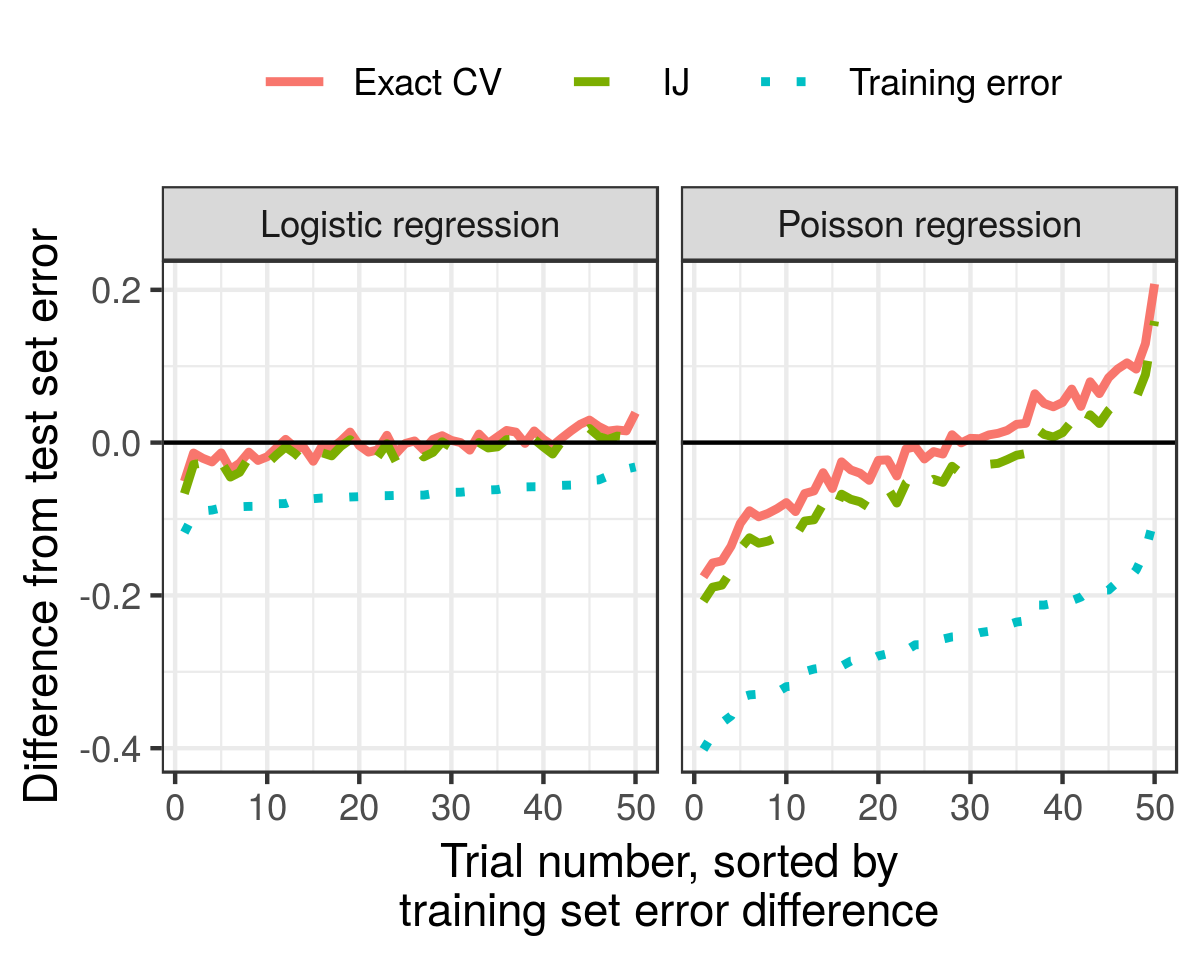
\includegraphics[width=0.98\linewidth,height=0.784\linewidth]{figure/simulated_experiments_accuracy-1} 

}

\caption[Simulated data]{Simulated data: accuracy results.}\label{fig:simulated_experiments_accuracy}
\end{figure}


\end{knitrout}
%
For a ground truth, we generate a large test set with $N=100{,}000$ datapoints
to measure the true generalization error. We show in
\fig{simulated_experiments_accuracy} that, over 50 randomly generated datasets,
our approximation consistently underestimates the actual error predicted by
exact leave-one-out CV; however, the difference is small relative to the
improvements they both make over the error evaluated on the training set.
%

\begin{knitrout}
\definecolor{shadecolor}{rgb}{0.969, 0.969, 0.969}\color{fgcolor}\begin{figure}[!h]

{\centering 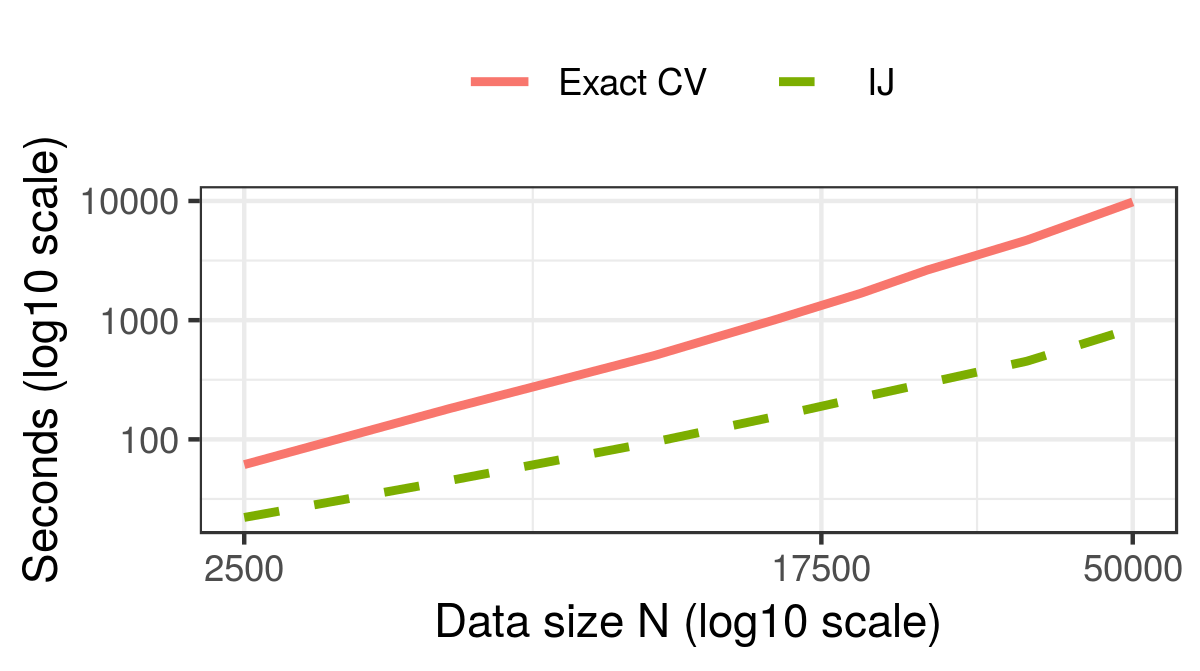
\includegraphics[width=0.98\linewidth,height=0.549\linewidth]{figure/simulated_experiments_timing-1} 

}

\caption[Simulated data]{Simulated data: timing results.}\label{fig:simulated_experiments_timing}
\end{figure}


\end{knitrout}
%
\fig{simulated_experiments_timing} shows the relative timings of our
approximation and exact leave-one-out CV on logistic regression with datasets of
increasing size. The time to run our approximation is roughly an order of
magnitude smaller.



\section{Genomics Experiments\label{sec:genomics}}
% This file is built with knit_real_data_to_tex.sh.
%%%%%%%%%%%%%%%%%%%%%%%%%%%%%%%%%%%%%%
%%%%%%%%%%%%%%%%%%%%%%%%%%%%%%%%%%%%%%
% Do not edit the TeX file your work
% will be overwritten.  Edit the RnW
% file instead.
%%%%%%%%%%%%%%%%%%%%%%%%%%%%%%%%%%%%%%
%%%%%%%%%%%%%%%%%%%%%%%%%%%%%%%%%%%%%%







\newcommand{\approxopttime}{42}
\newcommand{\approxhesstime}{360}
\newcommand{\fullparamdim}{39,000}


% TODO: define these in knitr instead.
\global\long\def\splinedegree{3}
\global\long\def\ntime{14}
\global\long\def\ngenes{1000}
\global\long\def\nclusters{18}
\global\long\def\covregularization{0.1}

We now consider a genomics application in which we use CV to choose the degree
of a spline smoother when clustering time series of gene expression data. Code and
instructions to reproduce our results can be found in the git repository
\href{https://github.com/rgiordan/AISTATS2019SwissArmyIJ}{rgiordan/AISTATS2019SwissArmyIJ}.
The application is also described in detail in \appsect{appendix_genomics}.

We use a publicly available data set of mice gene expression
\citep{shoemaker:2015:ultrasensitive} in which mice were infected with influenza
virus, and gene expression was assessed several times after infection. The
observed data consists of expression levels $y_{gt}$ for genes $g=1, \ldots,
n_{g}$ and time points $t=1, \ldots, n_{t}$.  In our case $n_{g}=\ngenes$ and
$n_{t}=\ntime$. Many genes behave the same way; thus, clustering the genes by
the pattern of their behavior over time allows dimensionality reduction that can
facilitate interpretation. Consequently, we wish to first fit a smoothed
regression line to each gene and then cluster the results. Following
\cite{Luan:2003:clustering}, we model the time series as a gene-specific
constant additive offset plus a B-spline basis of degree $\splinedegree$, and
the task is to choose the B-spline basis degrees of freedom using
cross-validation on the time points.

Our analysis runs in two stages---first, we regress the genes on the spline
basis, and then we cluster a transformed version of the regression fits. By
modeling in two stages, we both speed up the clustering and allow for the use of
flexible transforms of the fits. We are interested in choosing the smoothing
parameter using CV on the time points. Both the time points and the smoothing
parameter enter the regression objective directly, but they affect the
clustering objective only through the optimal regression parameters. Because the
optimization proceeds in two stages, the fit is not the optimum of any single
objective function.  However, it can still be represented as an M-estimator
(see \appsect{appendix_genomics}).

We implemented the model in \texttt{scipy} \citep{scipy} and computed all
derivatives with \texttt{autograd} \citep{maclaurin:2015:autograd}. We note that
the match between ``exact'' cross-validation (removing time points and
re-optimizing) and the IJ was considerably improved by
using a high-quality second-order optimization method.
% For more details,
% see \appsect{appendix_genomics}.
In particular, for these
experiments, we employed the Newton conjugate-gradient trust region method
\citep[Chapter 7.1]{wright:1999:optimization} as implemented by the method
\texttt{trust-ncg} in \texttt{scipy.optimize}, preconditioned by the Cholesky
decomposition of an inverse Hessian calculated at an initial approximate
optimum.
The Hessian used for the preconditioner was with respect to
the clustering parameters only and so could be calculated quickly, in contrast
to the $\hone$ matrix used for the IJ, which includes the
regression parameters as well.
 We found that first-order or quasi-Newton
methods (such as BFGS) often got stuck or terminated at points with fairly large
gradients. At such points our method does not apply in theory nor, we found,
very well in practice.
%

\begin{knitrout}
\definecolor{shadecolor}{rgb}{0.969, 0.969, 0.969}\color{fgcolor}\begin{figure}[!h]

{\centering 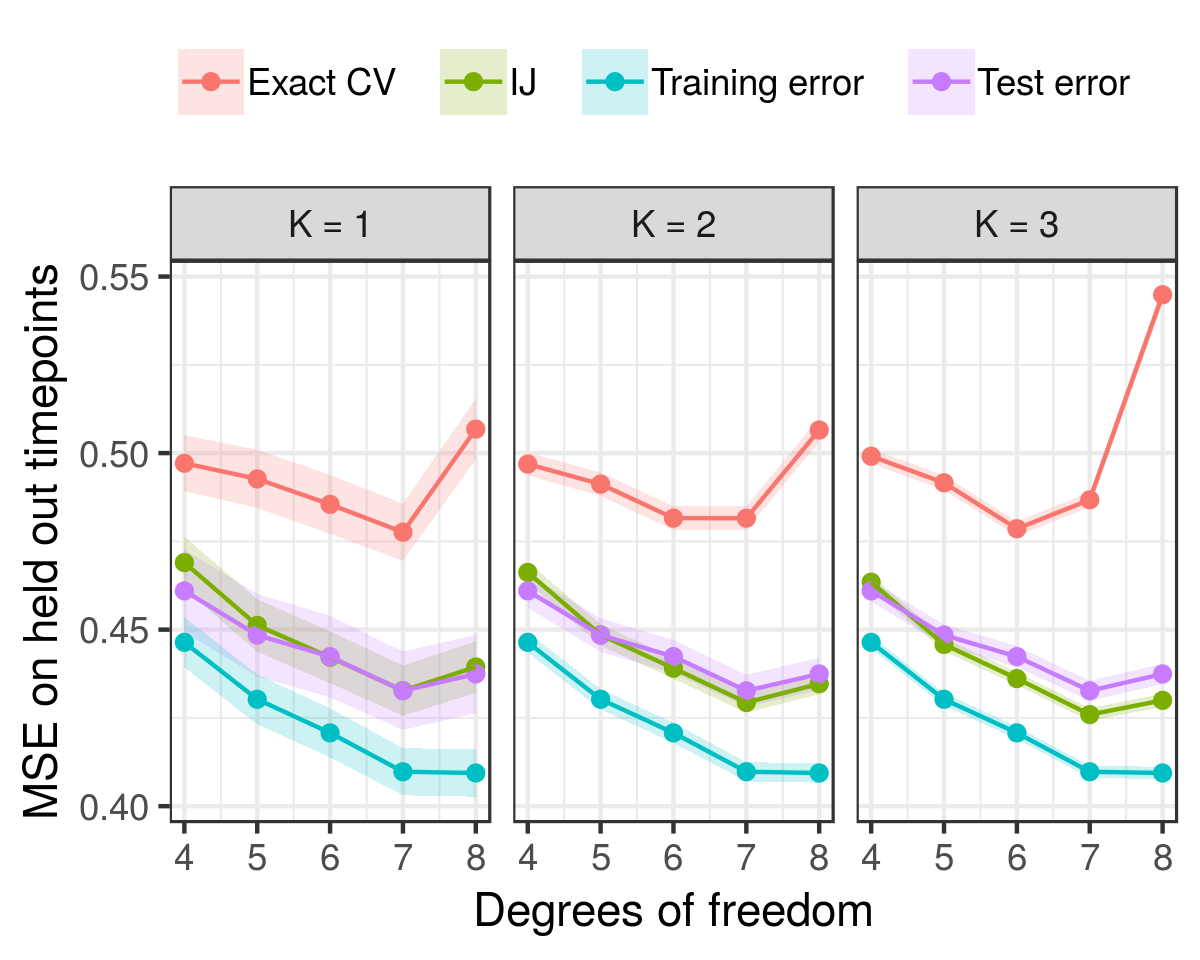
\includegraphics[width=0.98\linewidth,height=0.784\linewidth]{figure/mse_graph-1} 

}

\caption[Genomics data]{Genomics data: accuracy results.}\label{fig:mse_graph}
\end{figure}


\end{knitrout}
%
\fig{mse_graph} shows that the IJ is a reasonably good approximation to the test
set error.\footnote{In fact, in this case, the IJ is a better predictor of test
set error than exact CV.  However, the authors have no reason at present to
believe that the IJ is a better predictor of test error than exact CV in
general.} In particular, both the IJ and exact CV capture the increase in test
error for $df=8$, which is not present in the training error. Thus we see that,
like exact CV, the IJ is able to prevent overfitting. Though the IJ
underestimates exact CV, we note that it differs from exact CV by no more than
exact CV itself differs from the true quantity of iterest, the test error.
%

\begin{knitrout}
\definecolor{shadecolor}{rgb}{0.969, 0.969, 0.969}\color{fgcolor}\begin{figure}[!h]

{\centering 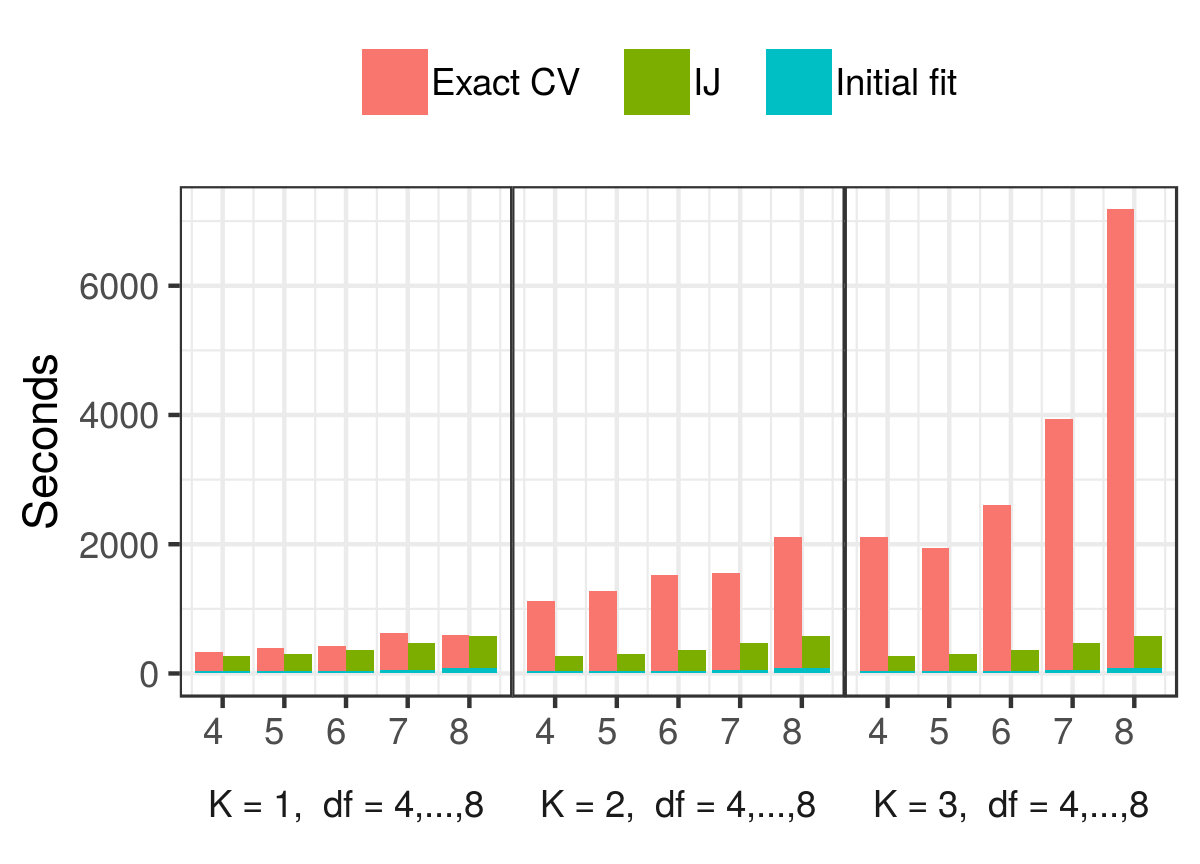
\includegraphics[width=0.98\linewidth,height=0.706\linewidth]{figure/timing_graph-1} 

}

\caption[Genomics data]{Genomics data: timing results.}\label{fig:timing_graph}
\end{figure}


\end{knitrout}
%
The timing results for the genomics experiment are shown in \fig{timing_graph}.
For this particular problem with approximately $\fullparamdim$ parameters (the
precise number depends on the degrees of freedom), finding the initial optimum
takes about $\approxopttime$ seconds. The cost of finding the initial optimum is
shared by exact CV and the IJ, and, as shown in
\fig{timing_graph}, is a small proportion of both.

The principle time cost of the IJ is the
computation of $\hone$. Computing and inverting a dense matrix of size
$\fullparamdim$ would be computationally prohibitive.
But, for the regression objective, $\hone$ is extremely sparse and block diagonal, so computing
$\hone$ in this case took only around $\approxhesstime$ seconds.  Inverting $\hone$
took negligible time. Once we have $\hone^{-1}$, obtaining the
subsequent IJ approximations is nearly instantaneous.

The cost of refitting the model for exact CV varies by degrees of freedom
(increasing degrees of freedom increases the number of parameters) and the
number of left-out points (an increasing number of left-out datapoints increases
the number of refits). As can be seen in \fig{timing_graph}, for low degrees of
freedom and few left-out points, the cost of re-optimizing is approximately the
same as the cost of computing $\hone$.  However, as the degrees of freedom and
number of left-out points grow, the cost of exact CV increases to as much as an
order of magnitude more than that of the IJ.



\section{Conclusion}
We recommend consideration of the Swiss Army infinitesimal jackknife for modern
machine learning problems.  The large size of modern data both increases the
need for fast approximations and renders such approximations more accurate.
Furthermore, modern automatic differentiation renders many past practical
difficulties obsolete. By stepping back from the strict requirements of
classical statistical theory, we can see that the value of the infinitesimal
jackknife extends beyond its traditional application areas, while retaining
desirable generality in other respects.


\newpage
\paragraph{Acknowledgements.} We thank anonymous reviewers for their helpful
comments and suggestions. We are grateful to Nelle Varoquaux for her help
with the genomics experiments. This research was supported in part by DARPA (FA8650-18-2-7832), an ARO
YIP award, an NSF CAREER award, and the CSAIL-MSR Trustworthy AI Initiative. Ryan Giordano was
supported by the Gordon and Betty Moore Foundation through Grant GBMF3834 and by
the Alfred P. Sloan Foundation through Grant 2013-10-27 to the University of
California, Berkeley. Runjing Liu was supported by the NSF Graduate Research
Fellowship.


\bibliography{references}
\bibliographystyle{plainnat}

\newpage
\onecolumn
\appendix

\newcommand{\globalassum}{Assumptions \ref{assu:paper_smoothness}---\ref{assu:paper_bounded} }

\section{Detailed assumptions, lemmas, and proofs\label{sec:appendix_proofs}}





\subsection{Tools}

We begin by stating two general propositions that will be useful.
First, we show that a version of Cauchy-Schwartz can be applied to
weighted sums of tensors.
\begin{prop}
\label{propref:tensor_cauchy_schwartz}Tensor array version of H{\"o}lder's
inequality. Let $w$ be an array of scalars and let $a=\left(a_{1},...,a_{N}\right)$
be an array of tensors, were each $a_{n}$ is indexed by $i=1,\ldots,D_{A}$
($i$ may be a multi-index---e.g., if $A$ is a $D\times D$ matrix,
then $i=\left(j,k\right)$, for $j,k\in\left[D\right]$ and $D_{A}=D^{2}$).
Let $p,q\in\left[1,\infty\right]$ be two numbers such that $p^{-1}+q^{-1}=1$.
Then
\begin{align*}
\norm{\frac{1}{N}\sum_{n=1}^{N}w_{n}a_{n}}_{1} & \le\frac{D_{A}^{\frac{1}{p}}}{N}\norm w_{p}\norm a_{q}.
\end{align*}
In particular, with $p=q=2$,
\begin{align*}
\norm{\frac{1}{N}\sum_{n=1}^{N}w_{n}a_{n}}_{1} & \le\sqrt{D_{A}}\frac{\norm w_{2}}{\sqrt{N}}\frac{\norm a_{2}}{\sqrt{N}}.
\end{align*}
\end{prop}
\begin{proof}
The conclusion follows from the ordinary H{\"o}lder's inequality
applied term-wise to $n$ and Jensen's inequality applied to the indices
$i$.

\begin{align*}
\norm{\frac{1}{N}\sum_{n=1}^{N}w_{n}a_{n}}_{1} & =\sum_{i=1}^{D_{A}}\left|\frac{1}{N}\sum_{n=1}^{N}w_{n}\left(a_{n}\right)_{i}\right|\\
 & \le\frac{1}{N}\sum_{i=1}^{D_{A}}\left|\left(\sum_{n=1}^{N}\left|w_{n}\right|^{p}\right)^{\frac{1}{p}}\left(\sum_{n=1}^{N}\left|\left(a_{n}\right)_{i}\right|^{q}\right)^{\frac{1}{q}}\right|\text{(H{\"o}lder)}\\
 & =\frac{1}{N}\norm w_{p}\frac{D_{A}}{D_{A}}\sum_{i=1}^{D_{A}}\left(\sum_{n=1}^{N}\left|\left(a_{n}\right)_{i}\right|^{q}\right)^{\frac{1}{q}}\\
 & \le\frac{1}{N}\norm w_{p}D_{A}\left(\frac{1}{D_{A}}\sum_{i=1}^{D_{A}}\sum_{n=1}^{N}\left|\left(a_{n}\right)_{i}\right|^{q}\right)^{\frac{1}{q}}\textrm{ (Jensen applied to }i\textrm{)}\\
 & =\frac{1}{N}\norm w_{p}D_{A}\left(\frac{1}{D_{A}}\sum_{n=1}^{N}\norm{a_{n}}_{q}^{q}\right)^{\frac{1}{q}}\\
 & =\frac{1}{N}\norm w_{p}D_{A}^{1-\frac{1}{q}}\norm a_{q}\\
 & =\frac{D_{A}^{\frac{1}{p}}}{N}\norm w_{p}\norm a_{q}.
\end{align*}
\end{proof}
%
Next, we prove a relationship between the term-wise difference between
matrices and the difference between their operator norms. It is well-known
that the minimum eigenvalue of a non-singular matrix is continuous
in the entries of the matrix. In the next proposition, we quantify
this continuity for the $L_{1}$ norm.
\begin{prop}
\label{propref:operator_norm_continuity}Let $A$ and $B$ be two
matrices. Let $\norm{A^{-1}}_{op}\le\constop$ for some finite $\constop$,
Then
\begin{align*}
\norm{A-B}_{1}\le\frac{1}{2}\constop[-1] & \quad\Rightarrow\quad\norm{B^{-1}}_{op}\le2\constop.
\end{align*}
\end{prop}
\begin{proof}
We will use \citet[Theorem 5.20]{schott:2016:matrix} and the associated
discussion, which states the following general result. Take any matrix
norm $\norm{\cdot}$ that satisfies $\norm I=1$, where $I$ is the
identity matrix. Then if $\norm{A^{-1}}\norm{A-B}<1$, then
\begin{align}
\norm{A^{-1}-\left(A-B\right)^{-1}} & \le\frac{\norm{A^{-1}}\norm{A-B}}{1-\norm{A^{-1}}\norm{A-B}}\norm{A^{-1}}.\label{eq:matrix_norm_continuity}
\end{align}

We will apply \eqref{matrix_norm_continuity} using the operator norm
$\norm{\cdot}_{op}$, for which $\norm I_{op}=1$. First, note that
\begin{align*}
\norm{A^{-1}}_{op}\norm{A-B}_{op} & \le\norm{A^{-1}}_{op}\norm{A-B}_{1}\textrm{ (ordering of matrix norms)}\\
 & \le\frac{1}{2}\constop\constop[-1]\\
 & =\frac{1}{2},
\end{align*}

so we can apply \eqref{matrix_norm_continuity}. Then
\begin{align*}
\norm{B^{-1}}_{op}
 & \le \norm{B^{-1}-A^{-1}}_{op}+\norm{A^{-1}}_{op}\textrm{ (triangle inequality)}\\
 & \le\frac{\norm{A^{-1}}_{op}\norm{A-B}_{op}}{1-\norm{A^{-1}}_{op}\norm{A-B}_{op}}\norm{A^{-1}}_{op}+\norm{A^{-1}}_{op}\textrm{ (Equation \ref{eq:matrix_norm_continuity})}\\
 & \le\left(\frac{\frac{1}{2}}{1-\frac{1}{2}}+1\right)\norm{A^{-1}}\\
 & \le2\constop.
\end{align*}
\end{proof}








\subsection{Lemmas}

We now prove some useful consequences of our assumptions. The proof
roughly proceeds for all $w\in W_{\delta}$ by the following steps:
\begin{enumerate}
\item When $\delta$ is small we can make $\norm{{{\thetaw}}-\thetaone}_{2}$
small. (\lemref{theta_difference_bound} below.)
\item When $\norm{\theta-\thetaone}_{2}$ is small, then the derivatives
$H\left(\theta,w\right)$ are close to their optimal value, $H\left(\thetaone,\onevec\right)$.
(\lemref{bounded_continuous} and \lemref{gh_difference_from_one}
below.)
\item When the derivatives are close to their optimal values, then $H\left(\theta,w\right)$
is uniformly non-singular. (\lemref{continuous_invertibility} below.)
\item When the derivatives are close to their optimal values and $H\left(\theta,w\right)$
is uniformly non-singular we can control the error in $\thetaij-\thetaw$
in terms of $\delta$. (\thmrefref{taylor_error_first} below.)
\end{enumerate}
We begin by showing that the difference between $\thetaw$ and $\thetaone$
for $w\in W_{\delta}$ can be made small by making $\delta$ from
\condref{paper_uniform_bound} small.

\begin{lem}
\label{lem:theta_difference_bound}Small parameter changes. Under
\globalassum and \condref{paper_uniform_bound},
\begin{align*}
\textrm{for all }w\in W_{\delta},\quad\norm{{{\thetaw}}-\thetaone}_{2} & \le\constop\delta.
\end{align*}
\end{lem}
\begin{proof}
By a first-order Taylor expansion in $\theta$, for some $\tilde{\theta}$
such that $\norm{\tilde{\theta}-\thetaone}_{2}\le\norm{{{\thetaw}}-\thetaone}_{2}$,
\begin{align*}
G\left(\thetaw,\onevec\right) & =G\left(\thetaone,\onevec\right)+H\left(\tilde{\theta},\onevec\right)\left(\thetaw-\thetaone\right).
\end{align*}
By \assuref{paper_hessian}, $H\left(\tilde{\theta},\onevec\right)$
is non-singular. A little manipulation, together with the fact that
$G\left(\thetaw,w\right)=G\left(\thetaone,\onevec\right)=0$ gives
\begin{align*}
G\left(\thetaw,\onevec\right)-G\left(\thetaw,w\right) & =H\left(\tilde{\theta},\onevec\right)\left(\thetaw-\thetaone\right)\Rightarrow\\
\thetaw-\thetaone & =H\left(\tilde{\theta},\onevec\right)^{-1}\left(G\left(\thetaw,\onevec\right)-G\left(\thetaw,w\right)\right).
\end{align*}
Applying \condref{paper_uniform_bound} and \assuref{paper_hessian},
\begin{align*}
\norm{{{\thetaw}}-\thetaone}_{2} & =\norm{H\left(\tilde{\theta},\onevec\right)^{-1}\left(G\left({{\thetaw}},\onevec\right)-G\left({{\thetaw}},w\right)\right)}_{2}\\
 & \le\norm{H\left(\tilde{\theta},\onevec\right)^{-1}}_{op}\norm{\left(G\left({{\thetaw}},\onevec\right)-G\left({{\thetaw}},w\right)\right)}_{2}\\
 & \le\sup_{\theta\in\Omega_{\theta}}\norm{H\left(\theta,\onevec\right)^{-1}}_{op}\norm{\left(G\left({{\thetaw}},\onevec\right)-G\left({{\thetaw}},w\right)\right)}_{2}\\
 & \le\constop\norm{G\left({{\thetaw}},\onevec\right)-G\left({{\thetaw}},w\right)}_{2}\textrm{ (Assumption \ref{assu:paper_hessian})}\\
 & \le\constop\norm{G\left({{\thetaw}},\onevec\right)-G\left({{\thetaw}},w\right)}_{1}\textrm{ (relation between norms)}\\
 & \le\constop\sup_{\theta\in\Omega_{\theta}}\norm{G\left(\theta,\onevec\right)-G\left(\theta,w\right)}_{1}\\
 & \le\constop\delta.\textrm{ (Condition \ref{cond:paper_uniform_bound}).}
\end{align*}
\end{proof}
%
Because we will refer to it repeatedly, we give the set of $\theta$
defined in \lemref{theta_difference_bound} a name.
\begin{defn}
For a given $\delta$, define the region around $\thetaone$ given
by \lemref{theta_difference_bound} as

\begin{align*}
\thetadeltaball & :=\left\{ \theta:\norm{\theta-\thetaone}_{2}\le\constop\delta\right\} \bigcap\Omega_{\theta}.
\end{align*}
\end{defn}
%
In other words, \lemref{theta_difference_bound} states that \condref{paper_uniform_bound}
implies $\thetaw\in\thetadeltaball$ when $w\in W_{\delta}$.

Next, we show that closeness in $\theta$ will mean closeness in $H\left(\theta,w\right)$.
\begin{lem}
\label{lem:bounded_continuous} Boundedness and continuity. Under
\paperallcoreassum and \condref{paper_uniform_bound},
\begin{align*}
\textrm{for all }\theta\in\thetaball,\quad\sup_{w\in W}\norm{H\left(\theta,w\right)-H\left(\thetaone,w\right)}_{1} & \le D\constw\liph\norm{\theta-\thetaone}_{2}.
\end{align*}
\end{lem}
\begin{proof}
For $\theta\in\thetaball$,
\begin{align*}
\sup_{w\in W}\norm{H\left(\theta,w\right)-H\left(\thetaone,w\right)}_{1} & =\sup_{w\in W}\norm{\frac{1}{N}\sum_{n=1}^{N}w_{n}\left(h_{n}\left(\theta\right)-h_{n}\left(\thetaone\right)\right)}_{1}\textrm{ (by definition)}\\
 & \le D\sup_{w\in W}\frac{\norm w_{2}}{\sqrt{N}}\frac{\norm{h\left(\theta\right)-h\left(\thetaone\right)}_{2}}{\sqrt{N}}\textrm{ (Proposition \ref{propref:tensor_cauchy_schwartz})}\\
 & \le D\constw\frac{\norm{h\left(\theta\right)-h\left(\thetaone\right)}_{2}}{\sqrt{N}}\textrm{ (Assumption \ref{assu:paper_weight_bounded})}\\
 & \le D\constw\liph\norm{\theta-\thetaone}_{2}\textrm{ (Assumption \ref{assu:paper_lipschitz} and }\theta\in\thetaball\textrm{)}.
\end{align*}
\end{proof}
%
We now combine \lemref{theta_difference_bound} and \lemref{bounded_continuous}
to show that $H\left(\theta,w\right)$ is close to its value at the
solution $H\left(\thetaone,\onevec\right)$ for sufficiently small
$\delta$ and for all $\theta\in\thetadeltaball$.
%
\begin{lem}
\label{lem:gh_difference_from_one}Bounds for difference in parameters.
Under \paperallcoreassum and \condref{paper_uniform_bound}, if $\delta\le\thetasize\constop[-1]$,
then
\begin{align*}
\sup_{\theta\in\thetadeltaball}\sup_{w\in W_{\delta}} & \norm{H\left(\theta,w\right)-H\left(\thetaone,\onevec\right)}_{1}\le\left(1+D\constw\liph\constop\right)\delta.
\end{align*}
\end{lem}
\begin{proof}
By \lemref{theta_difference_bound}, $\delta\le\thetasize\constop[-1]$
implies that $\constop\delta\le\thetasize$ and so $\thetadeltaball\subseteq\thetaball$.
Consequently, we can apply \lemref{bounded_continuous}:
\begin{align*}
\sup_{\theta\in\thetadeltaball}\sup_{w\in W_{\delta}}\norm{H\left(\theta,w\right)-H\left(\thetaone,w\right)}_{1} & \le\sup_{\theta\in\thetaball}\sup_{w\in W_{\delta}}\norm{H\left(\theta,w\right)-H\left(\thetaone,w\right)}_{1}\\
 & \le D\constw\liph\norm{\theta-\thetaone}_{2}\textrm{ (Lemma \ref{lem:bounded_continuous})}\\
 & \le D\constw\liph\constop\delta\quad\textrm{ (because }\theta\in\thetadeltaball\textrm{)}.
\end{align*}
%
Next, we can use this to write
\begin{align*}
\sup_{\theta\in\thetadeltaball}\sup_{w\in W_{\delta}} & \norm{H\left(\theta,w\right)-H\left(\thetaone,\onevec\right)}_{1}\\
 & =\sup_{\theta\in\thetadeltaball}\sup_{w\in W_{\delta}}\norm{H\left(\theta,w\right)-H\left(\theta,\onevec\right)+H\left(\theta,\onevec\right)-H\left(\thetaone,\onevec\right)}_{1}\\
 & \le\sup_{\theta\in\thetadeltaball}\sup_{w\in W_{\delta}}\norm{H\left(\theta,w\right)-H\left(\theta,\onevec\right)}_{1}+\sup_{\theta\in\thetadeltaball}\sup_{w\in W_{\delta}}\norm{H\left(\theta,\onevec\right)-H\left(\thetaone,\onevec\right)}_{1}\\
 & \le\sup_{\theta\in\Omega_{\theta}}\sup_{w\in W_{\delta}}\norm{H\left(\theta,w\right)-H\left(\theta,\onevec\right)}_{1}+\sup_{\theta\in\thetadeltaball}\sup_{w\in W_{\delta}}\norm{H\left(\theta,\onevec\right)-H\left(\thetaone,\onevec\right)}_{1}\\
 & \le\delta+\sup_{\theta\in\thetadeltaball}\sup_{w\in W_{\delta}}\norm{H\left(\theta,\onevec\right)-H\left(\thetaone,\onevec\right)}_{1}\textrm{ (Condition \ref{cond:paper_uniform_bound})}\\
 & \le\delta+D\constw\liph\constop\delta.
\end{align*}
\end{proof}
%
The constant that appears multiplying $\delta$ at the end of the proof of
\lemref{gh_difference_from_one} will appear often in what follows, so we give it
the special name $\constij$ in \defrefref{constants_definition}.

% \begin{defn}
% Define the constant that appears in the Hessian bound of \lemref{gh_difference_from_one}
% as
% \begin{align*}
% \constij & :=1+D\constw\liph\constop.
% \end{align*}
% \end{defn}
%
Note that \lemref{gh_difference_from_one} places a condition on how
small $\delta$ must be in order for our regularity conditions to
apply. \lemref{theta_difference_bound} will guarantee that $\thetaw\in\thetadeltaball$,
but if we are not able to make $\delta$ arbitrarily small in \condref{paper_uniform_bound},
then we are not guaranteed to ensure that $\thetadeltaball\subseteq\thetaball$,
will not be able to assume Lipschitz continuity, and none of our results
will apply.

Next, using \lemref{gh_difference_from_one}, we can extend the operator
bound on $\hone^{-1}$ from \assuref{paper_hessian} to $H\left(\theta,w\right)^{-1}$
for all $w\in W_{\delta}$, not only for $w=\onevec$.

\begin{lem}
\label{lem:continuous_invertibility}Uniform invertibility of the
Hessian. Under \paperallcoreassum and \condref{paper_uniform_bound}, if $\delta\le\min\left\{ \thetasize\constop[-1],\frac{1}{2}\constij^{-1}\constop[-1]\right\} $,
then
\begin{align*}
\sup_{\theta\in\thetadeltaball}\sup_{w\in W_{\delta}}\norm{H\left(\theta,w\right)^{-1}}_{op} & \le2\constop.
\end{align*}
\end{lem}
\begin{proof}
By \assuref{paper_hessian}, $\norm{H\left(\thetaone,\onevec\right)^{-1}}_{op}\le\constop$.
So by \proprefref{operator_norm_continuity}, it will suffice to select
$\delta$ so that
\begin{align}
\sup_{\theta\in\thetadeltaball}\sup_{w\in W_{\delta}}\norm{H\left(\theta,w\right)-H\left(\thetaone,\onevec\right)}_{1} & \le\frac{1}{2}\constop[-1].\label{eq:h_bound}
\end{align}
When we can apply \lemref{gh_difference_from_one}, we have
\begin{align*}
\sup_{\theta\in\thetadeltaball}\sup_{w\in W_{\delta}}\norm{H\left(\theta,w\right)-H\left(\thetaone,\onevec\right)}_{1} & \le\constij\delta.
\end{align*}
So $H\left(\theta,w\right)$ will satisfy \eqref{h_bound} if we can
apply \lemref{gh_difference_from_one} and if
\begin{align*}
\delta\le & \frac{1}{2}\constop[-1]\constij^{-1}.
\end{align*}
To apply \lemref{gh_difference_from_one} we additionally require
that $\delta\le\thetasize\constop[-1]$. By taking $\delta\le\min\left\{ \thetasize\constop[-1],\frac{1}{2}\constop[-1]\constij^{-1}\right\} $,
we satisfy \eqref{h_bound} and the result follows.
\end{proof}
%
At last, the upper bound on $\delta$ will be sufficient to control
the error terms in our approximation. For compactness, we give it
the name $\deltasize$ in \defrefref{constants_definition}.
% \begin{defn}
% Define $\deltasize$ as the upper bound on $\delta$ given by \lemref{continuous_invertibility}.
% \begin{align*}
% \deltasize & :=\min\left\{ \thetasize\constop[-1],\frac{1}{2}\constop[-1]\constij^{-1}\right\} .
% \end{align*}
%
%\end{defn}

Finally, we state a result that will allow us to define derivatives
of $\thetaw$ with respect to $w$.
\begin{lem}
\label{lem:implicit_function_theorem}Inverse function theorem. Under
\paperallcoreassum and \condref{paper_uniform_bound}, and for $\delta\le\deltasize$,
there exists a continuous, differentiable function of $w$, $\thetahat\left(w\right)$,
such that, for all $w\in W$, G$\left(\thetahat\left(w\right),w\right)=0$.
\end{lem}
\begin{proof}
This follows from \lemref{continuous_invertibility} and the implicit
function theorem.
\end{proof}
By definition, $\thetahat\left(\onevec\right)=\thetaone$.






\subsection{Bounding the errors in a Taylor expansion}

We are now in a position to use \paperallcoreassum and \condref{paper_uniform_bound}
to bound the error terms in a first-order Taylor expansion of $\thetaw$.
We begin by simply calculating the derivative $d\thetahat\left(w\right)/dw$.
\begin{prop}
\label{propref:theta_w_first_derivative}For any $w\in W$ for which
$H\left(\thetaw,w\right)$ is invertible, and for any vector $a\in\mathbb{R}^{N}$,
\begin{align*}
\frac{d\thetaw}{dw^{T}}\at wa & =-H\left(\thetaw,w\right)^{-1}G\left(\thetaw,a\right).
\end{align*}
\end{prop}
\begin{proof}
Because $G\left(\thetaw,w\right)=0$ for all $w\in W$, by direct
calculation,
\begin{align*}
0 & =\frac{d}{dw^{T}}G\left(\thetaw,w\right)\at wa\\
 & =\left(\frac{\partial G}{\partial\theta^{T}}\frac{d\hat{\theta}}{dw^{T}}+\frac{\partial G}{\partial w^{T}}\right)\at{_{w}}a\\
 & =H\left(\thetaw,w\right)\frac{d\hat{\theta}}{dw^{T}}\at{_{w}}a+\left(\frac{\partial}{\partial w^{T}}\frac{1}{N}\sum_{n=1}^{N}w_{n}g_{n}\left(\theta\right)\right)\at{_{w}}a\\
 & =H\left(\thetaw,w\right)\frac{d\hat{\theta}}{dw^{T}}\at{_{w}}a+\frac{1}{N}\sum_{n=1}^{N}g_{n}\left(\thetaw\right)a\\
 & =H\left(\thetaw,w\right)\frac{d\hat{\theta}}{dw^{T}}\at{_{w}}a+G\left(\thetaw,a\right).
\end{align*}
Because $H\left(\thetaw,w\right)$ is invertible by assumption, the
result follows.
\end{proof}
\begin{defn}
\label{defref:theta_infinitesimal_jackknife}Define
\begin{align*}
\thetaij\left(w\right) & :=\thetaone+\frac{d\thetaw}{dw^{T}}\at{\onevec}\left(w-\onevec\right)\\
 & =\thetaone-\hone^{-1}G\left(\thetaone,w\right).\textrm{ (because }G\left(\thetaone,\onevec\right)=0\textrm{)}
\end{align*}
\end{defn}
%
$\thetaij\left(w\right)$ in \defrefref{theta_infinitesimal_jackknife}
is the first term in a Taylor series expansion of $\thetaw$ as a
function of $w$. We want to bound the error, $\thetaij\left(w\right)-\thetaw$.
\begin{thm}
\label{thmref:taylor_error_first}Under \paperallcoreassum and \condref{paper_uniform_bound},
when $\delta\le\deltasize$,
\begin{align*}
\sup_{w\in W_{\delta}}\norm{\thetaij\left(w\right)-\thetahat\left(w\right)}_{2} & \le2\constop[2]\constij\delta^{2}.
\end{align*}
\end{thm}
\begin{proof}
By a one-term Taylor series expansion of $G\left(\thetaw,w\right)=0$
in $\theta$ around $\thetaone$, we have, for some $\thetawiggle$
such that $\norm{\thetawiggle-\thetaone}_{2}\le\norm{{{\thetaw}}-\thetaone}_{2}$,
\begin{align*}
0=G\left(\thetaw,w\right) & =G\left(\thetaone,w\right)+H\left(\thetawiggle,w\right)\left(\thetaw[w]-\thetaone\right).
\end{align*}
Because $\delta\in W_{\delta}$, \lemref{theta_difference_bound}
implies that $\thetaw\in\thetadeltaball$. Because $\norm{\thetawiggle-\thetaone}_{2}\le\norm{{{\thetaw}}-\thetaone}_{2}$,
$\thetawiggle\in\thetadeltaball$ as well. Because $\thetawiggle\in\thetadeltaball$,
\lemref{continuous_invertibility} implies that $H\left(\thetawiggle,w\right)$
is invertible, so we can solve for $\thetaw-\thetaone$.
\begin{align*}
\thetaw[w]-\thetaone & =-H\left(\thetawiggle,w\right)^{-1}G\left(\thetaone,w\right)\\
 & =\left(-H\left(\thetawiggle,w\right)^{-1}+H\left(\thetaone,\onevec\right)^{-1}-H\left(\thetaone,\onevec\right)^{-1}\right)G\left(\thetaone,w\right)\\
 & =\left(H\left(\thetaone,\onevec\right)^{-1}-H\left(\thetawiggle,w\right)^{-1}\right)G\left(\thetaone,w\right)+\thetaij\left(w\right)-\thetaone.
\end{align*}
Eliminating $\thetaone$ and taking the supremum of both sides we
have that
\begin{align*}
\sup_{w\in W_{\delta}} & \norm{\thetaij\left(w\right)-{{\thetaw[w]}}}_{2}\\
 & =\sup_{w\in W_{\delta}}\norm{\left(H\left(\thetaone,\onevec\right)^{-1}-H\left(\thetawiggle,w\right)^{-1}\right)G\left(\thetaone,w\right)}_{2}\\
 & =\sup_{w\in W_{\delta}}\norm{H\left(\thetawiggle,w\right)^{-1}\left(H\left(\thetawiggle,w\right)-H\left(\thetaone,\onevec\right)\right)H\left(\thetaone,\onevec\right)^{-1}G\left(\thetaone,w\right)}_{2}\\
 & \le2\constop\sup_{w\in W_{\delta}}\norm{\left(H\left(\thetawiggle,w\right)-H\left(\thetaone,\onevec\right)\right)H\left(\thetaone,\onevec\right)^{-1}G\left(\thetaone,w\right)}_{2}\textrm{ (Lemma \ref{lem:continuous_invertibility})}\\
 & \le2\constop\sup_{w\in W_{\delta}}\norm{H\left(\thetawiggle,w\right)-H\left(\thetaone,\onevec\right)}_{op}\norm{H\left(\thetaone,\onevec\right)^{-1}G\left(\thetaone,w\right)}_{2}\\
 & \le2\constop\sup_{w\in W_{\delta}}\norm{H\left(\thetawiggle,w\right)-H\left(\thetaone,\onevec\right)}_{2}\norm{H\left(\thetaone,\onevec\right)^{-1}G\left(\thetaone,w\right)}_{2}\textrm{ (ordering of matrix norms)}\\
 & \le2\constop\constij\delta\sup_{w\in W_{\delta}}\norm{H\left(\thetaone,\onevec\right)^{-1}G\left(\thetaone,w\right)}_{2}\textrm{ (Lemma \ref{lem:gh_difference_from_one})}\\
 & \le2\constop[2]\constij\delta\sup_{w\in W_{\delta}}\norm{G\left(\thetaone,w\right)}_{2}\textrm{ (Assumption \ref{assu:paper_hessian})}\\
 & =2\constop[2]\constij\delta\sup_{w\in W_{\delta}}\norm{G\left(\thetaone,w\right)-G\left(\thetaone,\onevec\right)}_{2}\textrm{ (because }G\left(\thetaone,\onevec\right)=0\textrm{)}\\
 & \le2\constop[2]\constij\delta^{2}\textrm{ (Condition \ref{cond:paper_uniform_bound})}.
\end{align*}
\end{proof}
%






\subsection{Use cases\label{sec:use_cases}}

First, let us state a simple condition under which \coreassum
hold. It will help to have a lemma for the Lipschitz continuity.
\begin{lem}
Derivative Cauchy Schwartz. Let $a\left(\theta\right)=\left(a_{1}\left(\theta\right),...,a_{N}\left(\theta\right)\right)$
be an array of tensors with multi-index $i\in\left[D_{A}\right]$,
and let $\frac{\partial a\left(\theta\right)}{\partial\theta}=\left(\frac{\partial}{\partial\theta}a_{1}\left(\theta\right),...,\frac{\partial}{\partial\theta}a_{N}\left(\theta\right)\right)$
be an array of tensors of size $D\times D_{A}$. Then
\begin{align*}
\norm{\frac{\partial}{\partial\theta}\norm{a\left(\theta\right)}_{2}}_{2} & \le D_{A}\norm{\frac{\partial a}{\partial\theta}}_{2}.
\end{align*}
\end{lem}
\begin{proof}
By direct calculation,
\begin{align*}
\norm{\frac{\partial}{\partial\theta}\norm{a\left(\theta\right)}_{2}^{2}}_{2}^{2} & =\sum_{r=1}^{D}\left(\frac{\partial}{\partial\theta_{r}}\sum_{n=1}^{N}\sum_{i=1}^{D_{A}}a_{n,i}\left(\theta\right)^{2}\right)^{2}\\
 & =\sum_{r=1}^{D}\left(\sum_{n=1}^{N}\sum_{i=1}^{D_{A}}2a_{n,i}\left(\theta\right)\frac{\partial a_{n,i}\left(\theta\right)}{\partial\theta_{r}}\right)^{2}\\
 & \le\sum_{r=1}^{D}\left(2\sum_{i=1}^{D_{A}}\left(\sum_{n=1}^{N}a_{n,i}\left(\theta\right)^{2}\right)^{\frac{1}{2}}\left(\sum_{n=1}^{N}\left(\frac{\partial a_{n,i}\left(\theta\right)}{\partial\theta_{r}}\right)^{2}\right)^{\frac{1}{2}}\right)^{2}\\
 & \le\sum_{r=1}^{D}\left(2D_{A}^{2}\left(\frac{1}{D_{A}}\sum_{i=1}^{D_{A}}\sum_{n=1}^{N}a_{n,i}\left(\theta\right)^{2}\right)^{\frac{1}{2}}\left(\frac{1}{D_{A}}\sum_{n=1}^{N}\left(\frac{\partial a_{n,i}\left(\theta\right)}{\partial\theta_{r}}\right)^{2}\right)^{\frac{1}{2}}\right)^{2}\\
 & =4D_{A}^{2}\norm a_{2}^{2}\sum_{r=1}^{D}\norm{\frac{\partial a}{\partial\theta_{r}}}_{2}^{2}\\
 & =4D_{A}^{2}\norm a_{2}^{2}\norm{\frac{\partial a}{\partial\theta}}_{2}^{2}.
\end{align*}
By the chain rule,
\begin{align*}
\norm{\frac{\partial}{\partial\theta}\norm{a\left(\theta\right)}_{2}}_{2}^{2} & =\frac{1}{4\norm{a\left(\theta\right)}_{2}^{2}}\norm{\frac{\partial}{\partial\theta}\norm{a\left(\theta\right)}_{2}^{2}}_{2}^{2}\le D_{A}^{2}\norm{\frac{\partial a}{\partial\theta}}_{2}^{2}.
\end{align*}
\end{proof}
%
\begin{lem}
\label{lem:lipschitz_helper}Let $a\left(\theta\right)\in\mathbb{R}^{D\times D}$
be a continuously differentiable random matrix with a $D\times D\times D$
derivative tensor. (Note that the function, not $\theta$, is random.
For example, $\mbe\left[a\left(\theta\right)\right]$ is still a function
of $\theta$.) Suppose that $\mbe\left[\norm{a\left(\theta\right)}_{2}\right]$
is finite for all $\theta\in\Omega_{\theta}$. Then, for all $\theta_{1},\theta_{2}\in\Omega_{\theta}$,
\begin{align*}
\left|\mbe\left[\norm{a\left(\theta_{1}\right)}_{2}\right]-\mbe\left[\norm{a\left(\theta_{2}\right)}_{2}\right]\right| & \le\sqrt{\mbe\left[\sup_{\theta\in\Omega_{\theta}}\norm{\frac{\partial a\left(\theta\right)}{\partial\theta}}_{2}^{2}\right]}\norm{\theta_{1}-\theta_{2}}_{2}.
\end{align*}
\end{lem}
\begin{proof}
For any tensor $a$ with multi-index $i$,
\begin{align*}
\norm{\frac{\partial}{\partial\theta}\norm a_{2}^{2}}_{2}^{2} & =\sum_{r=1}^{D}\left(\frac{\partial}{\partial\theta_{r}}\norm a_{2}^{2}\right)^{2}\\
 & =\sum_{r=1}^{D}\left(\frac{\partial}{\partial\theta_{r}}\sum_{i=1}^{D_{A}}a_{i}^{2}\right)^{2}\\
 & =\sum_{r=1}^{D}\left(2\sum_{i=1}^{D_{A}}a_{i}\frac{\partial a_{i}}{\partial\theta_{r}}\right)^{2}\\
 & \le4\sum_{r=1}^{D}\sum_{i=1}^{D_{A}}a_{i}^{2}\sum_{i=1}^{D_{A}}\left(\frac{\partial a_{i}}{\partial\theta_{r}}\right)^{2}\textrm{ (Cauchy-Schwartz)}\\
 & =4\sum_{i=1}^{D_{A}}a_{i}^{2}\sum_{r=1}^{D}\sum_{i=1}^{D_{A}}\left(\frac{\partial a_{i}}{\partial\theta_{r}}\right)^{2}\\
 & =4\norm a_{2}^{2}\norm{\frac{\partial a}{\partial\theta}}_{2}^{2}.
\end{align*}

Consequently,
\begin{align*}
\norm{\frac{\partial}{\partial\theta}\norm{a\left(\theta\right)}_{2}}_{2}^{2} & =\norm{\frac{1}{2\norm{a\left(\theta\right)}_{2}}\frac{\partial}{\partial\theta}\norm{a\left(\theta\right)}_{2}^{2}}_{2}^{2}\\
 & =\frac{1}{4\norm{a\left(\theta\right)}_{2}^{2}}\norm{\frac{\partial}{\partial\theta}\norm{a\left(\theta\right)}_{2}^{2}}_{2}^{2}\\
 & \le\frac{4\norm{a\left(\theta\right)}_{2}^{2}}{4\norm{a\left(\theta\right)}_{2}^{2}}\norm{\frac{\partial}{\partial\theta}a\left(\theta\right)}_{2}^{2}\\
 & =\norm{\frac{\partial a\left(\theta\right)}{\partial\theta}}_{2}^{2}.
\end{align*}
So for any $\theta_{1},\theta_{2}\in\Omega_{\theta}$,
\begin{align*}
\left|\mbe\left[\norm{a\left(\theta_{1}\right)}_{2}\right]-\mbe\left[\norm{a\left(\theta_{2}\right)}_{2}\right]\right| & \le\mbe\left[\left|\norm{a\left(\theta_{1}\right)}_{2}-\norm{a\left(\theta_{2}\right)}_{2}\right|\right]\\
 & \le\mbe\left[\left(\sup_{\theta\in\Omega_{\theta}}\norm{\frac{\partial}{\partial\theta}\norm{a\left(\theta\right)}_{2}}_{2}\right)\right]\norm{\theta_{1}-\theta_{2}}_{2}\textrm{ (}\theta\textrm{ is not random)}\\
 & \le\mbe\left[\left(\sup_{\theta\in\Omega_{\theta}}\norm{\frac{\partial a\left(\theta\right)}{\partial\theta}}_{2}\right)\right]\norm{\theta_{1}-\theta_{2}}_{2}\\
 & \le\sqrt{\mbe\left[\sup_{\theta\in\Omega_{\theta}}\norm{\frac{\partial a\left(\theta\right)}{\partial\theta}}_{2}^{2}\right]}\norm{\theta_{1}-\theta_{2}}_{2}.
\end{align*}
The result follows. Note that the bound still holds (though vacuously)
if $\mbe\left[\sup_{\theta\in\Omega_{\theta}}\norm{\frac{\partial a\left(\theta\right)}{\partial\theta}}_{2}^{2}\right]$
is infinite.
\end{proof}
\begin{prop}
\label{prop:assumptions_hold}Let $\Omega_{\theta}$ be a compact
set. Let $g_{n}\left(\theta\right)$ be twice continuously differentiable
IID random functions. Define
\begin{align*}
h_{n}\left(\theta\right) & :=\frac{\partial g{}_{n}\left(\theta\right)}{\partial\theta}\\
r_{n}\left(\theta\right) & :=\frac{\partial^{2}g{}_{n}\left(\theta\right)}{\partial\theta\partial\theta},
\end{align*}
where $r_{n}\left(\theta\right)$ is a $D\times D\times D$ tensor.
Assume that

1a) $\mbe\left[\sup_{\theta\in\Omega_{\theta}}\norm{g_{n}\left(\theta\right)}_{2}^{2}\right]<\infty$;

1b) $\mbe\left[\sup_{\theta\in\Omega_{\theta}}\norm{h_{n}\left(\theta\right)}_{2}^{2}\right]<\infty$;

1c) $\mbe\left[\sup_{\theta\in\Omega_{\theta}}\norm{r_{n}\left(\theta\right)}_{2}^{2}\right]<\infty;$

2) $\mbe\left[h_{n}\left(\theta\right)\right]$ is non-singular for
all $\theta\in\Omega_{\theta}$;

3) We can exchange expectation and differentiation.

Then $\lim_{N\rightarrow\infty}P\left(\textrm{\coreassum\ hold}\right)=1.$
\end{prop}
%
\begin{proof}
    %
The proof follows from Theorems 9.1 and
9.2 of \citet{keener:2011:theoretical}. We will first show that the expected values of
the needed functions satisfy \coreassum, and then that the sample versions
converge uniformly.

By Jensen's inequality,
\begin{align*}
\mbe\left[\sup_{\theta\in\Omega_{\theta}}\norm{g_{n}\left(\theta\right)}_{2}\right] & =\mbe\left[\sqrt{\sup_{\theta\in\Omega_{\theta}}\norm{g_{n}\left(\theta\right)}_{2}^{2}}\right]\le\sqrt{\mbe\left[\sup_{\theta\in\Omega_{\theta}}\norm{g_{n}\left(\theta\right)}_{2}^{2}\right]}.
\end{align*}
Also, for the $i^{th}$ component of $g_{n}\left(\theta\right)$
\begin{align*}
\mbe\left[\sup_{\theta\in\Omega_{\theta}}\left|g_{n,i}\left(\theta\right)\right|\right] & \le\mbe\left[\sup_{\theta\in\Omega_{\theta}}\norm{g_{n}\left(\theta\right)}_{\infty}\right]\le\mbe\left[\sup_{\theta\in\Omega_{\theta}}\norm{g_{n}\left(\theta\right)}_{2}\right].
\end{align*}
By Theorem 9.1 of \citet{keener:2011:theoretical}, $\mbe\left[\norm{g_{n}\left(\theta\right)}_{2}^{2}\right]$
, $\mbe\left[\norm{g_{n}\left(\theta\right)}_{2}\right]$, and $\mbe\left[g_{n}\left(\theta\right)\right]$
are continuous functions of $\theta$, and because $\Omega_{\theta}$
is compact, they are each bounded. Similar reasoning applies to $h_{n}\left(\theta\right)$
and $r_{n}\left(\theta\right)$. Consequently we can define
\begin{align*}
\sup_{\theta\in\Omega_{\theta}}\mbe\left[\norm{g_{n}\left(\theta\right)}_{2}^{2}\right] & =:Q_{g}^{2}<\infty\\
\sup_{\theta\in\Omega_{\theta}}\mbe\left[\norm{h_{n}\left(\theta\right)}_{2}^{2}\right] & =:Q_{h}^{2}<\infty.
\end{align*}
Below, these constants will be used to satisfy \assuref{paper_smoothness}
and \assuref{paper_bounded} with high probability.

Because $\Omega_{\theta}$ is compact, $\mbe\left[h_{n}\left(\theta\right)\right]$
is continuous, $\mbe\left[h_{n}\left(\theta\right)\right]$ is non-singular,
and the operator norm is a continuous function of $\mbe\left[h_{n}\left(\theta\right)\right]$,
we can also define
\begin{align*}
\sup_{\theta\in\Omega_{\theta}}\norm{\mbe\left[h_{n}\left(\theta\right)\right]^{-1}}_{op} & =:Q_{op}<\infty.
\end{align*}
Below, this constant be used to satisfy \assuref{paper_hessian}
with high probability.

Finally, we turn to the Lipschitz condition. \lemref{lipschitz_helper}
implies that
\begin{align*}
\left|\mbe\left[\norm{h_{n}\left(\theta_{1}\right)}_{2}\right]-\mbe\left[\norm{h_{n}\left(\theta_{2}\right)}_{2}\right]\right| & \le\sqrt{\mbe\left[\sup_{\theta\in\Omega_{\theta}}\norm{r_{n}\left(\theta\right)}_{2}^{2}\right]}\norm{\theta_{1}-\theta_{2}}_{2}.
\end{align*}
Define
\begin{align*}
\Lambda_{h} & =\sqrt{\mbe\left[\sup_{\theta\in\Omega_{\theta}}\norm{r_{n}\left(\theta\right)}_{2}^{2}\right]},
\end{align*}
so that we have shown that $\mbe\left[\norm{h_{n}\left(\theta\right)}_{2}\right]$
is Lipschitz in $\Omega_{\theta}$ with constant $\Lambda_{h}$, which
is finite by assumption.

We have now shown, essentially, that the expected versions of the
quantities we wish to control satisfy \coreassum with $N=1$.
We now need to show that the sample versions satisfy \coreassum
with high probability, which will follow from the fact that the sample
versions converge uniformly to their expectations by
Theorem 9.2 of \citet{keener:2011:theoretical}.

First, observe that \assuref{paper_smoothness} holds with probability
one by assumption. For the remaining assumption choose an $\epsilon>0$,
and define
\begin{align*}
\constg & :=\sqrt{Q_{g}^{2}+\epsilon}\\
\consth & :=\sqrt{Q_{h}^{2}+\epsilon}\\
\constop & :=2Q_{op}\\
\liph & :=\sqrt{D^{4}\Lambda_{h}^{2}+\epsilon}.
\end{align*}

By \citet{keener:2011:theoretical} Theorem 9.2,
\begin{align*}
\sup_{\theta\in\Omega_{\theta}}\left|\frac{1}{N}\sum_{n=1}^{N}\norm{g_{n}\left(\theta\right)}_{2}^{2}-\mbe\left[\norm{g_{n}\left(\theta\right)}_{2}^{2}\right]\right| & \xrightarrow[N\rightarrow\infty]{p}0.
\end{align*}
Because
\begin{align*}
\sup_{\theta\in\Omega_{\theta}}\left|\frac{1}{N}\sum_{n=1}^{N}\norm{g_{n}\left(\theta\right)}_{2}^{2}\right| & >Q_{g}^{2}+\epsilon\ge\sup_{\theta\in\Omega_{\theta}}\mbe\left[\norm{g_{n}\left(\theta\right)}_{2}^{2}\right]+\epsilon\Rightarrow\\
\sup_{\theta\in\Omega_{\theta}}\left|\frac{1}{N}\sum_{n=1}^{N}\norm{g_{n}\left(\theta\right)}_{2}^{2}-\mbe\left[\norm{g_{n}\left(\theta\right)}_{2}^{2}\right]\right| & >\epsilon,
\end{align*}

we have
\begin{align*}
 & P\left(\sup_{\theta\in\Omega_{\theta}}\left|\frac{1}{N}\sum_{n=1}^{N}\norm{g_{n}\left(\theta\right)}_{2}^{2}\right|\ge Q_{g}^{2}+\epsilon\right)\le\\
 & \quad P\left(\sup_{\theta\in\Omega_{\theta}}\left|\frac{1}{N}\sum_{n=1}^{N}\norm{g_{n}\left(\theta\right)}_{2}^{2}-\mbe\left[\norm{g_{n}\left(\theta\right)}_{2}^{2}\right]\right|\le\epsilon\right),
\end{align*}
so
\begin{align*}
P\left(\sup_{\theta\in\Omega_{\theta}}\left|\frac{1}{N}\sum_{n=1}^{N}\norm{g_{n}\left(\theta\right)}_{2}^{2}\right|\ge\constg^{2}\right) & \xrightarrow[N\rightarrow\infty]{}0.
\end{align*}
An analogous argument holds for $\frac{1}{N}\norm{h_{n}\left(\theta\right)}_{2}^{2}$.
Consequently, $P\left(\textrm{Assumption \ref{assu:paper_bounded} holds}\right)\xrightarrow[N\rightarrow\infty]{}1$.

We now consider \assuref{paper_hessian}. Again, by \citet{keener:2011:theoretical} Theorem 9.2
applied to each element of the matrix $h_{n}\left(\theta\right)$,
using a union bound over each of the $D^{2}$ entries,
\begin{align*}
\sup_{\theta\in\Omega_{\theta}}\norm{\frac{1}{N}\sum_{n=1}^{N}h_{n}\left(\theta\right)-\mbe\left[h_{n}\left(\theta\right)\right]}_{1} & \xrightarrow[N\rightarrow\infty]{p}0.
\end{align*}
By the converse of \proprefref{operator_norm_continuity}, because
$\norm{\mbe\left[h_{n}\left(\theta\right)\right]^{-1}}_{op}\le Q_{op}$,
\begin{align*}
\norm{\left(\frac{1}{N}\sum_{n=1}^{N}h_{n}\left(\theta\right)\right)^{-1}}_{op} & >2Q_{op}=\constop\Rightarrow\\
\norm{\frac{1}{N}\sum_{n=1}^{N}h_{n}\left(\theta\right)-\mbe\left[h_{n}\left(\theta\right)\right]}_{1} & >\frac{1}{2}Q_{op}^{-1}.
\end{align*}
Consequently,
\begin{align*}
 & P\left(\norm{\left(\frac{1}{N}\sum_{n=1}^{N}h_{n}\left(\theta\right)\right)^{-1}}_{op}\ge\constop\right)\le\\
 & \quad P\left(\norm{\frac{1}{N}\sum_{n=1}^{N}h_{n}\left(\theta\right)-\mbe\left[h_{n}\left(\theta\right)\right]}_{1}\right)\xrightarrow[N\rightarrow\infty]{p}0,
\end{align*}
and $P\left(\textrm{Assumption \ref{assu:paper_hessian} holds}\right)\xrightarrow[N\rightarrow\infty]{}1.$

Finally, applying \lemref{lipschitz_helper} to $\frac{1}{\sqrt{N}}\norm{h\left(\theta_{2}\right)}_{2}$,
\begin{align*}
\left|\frac{1}{\sqrt{N}}\norm{h\left(\theta_{1}\right)}_{2}-\frac{1}{\sqrt{N}}\norm{h\left(\theta_{2}\right)}_{2}\right| & \le\sup_{\theta\in\Omega_{\theta}}\norm{\frac{\partial}{\partial\theta}\frac{1}{\sqrt{N}}\norm{h\left(\theta\right)}_{2}}_{2}\norm{\theta_{1}-\theta_{2}}_{2}\\
 & \le\frac{D^{2}}{\sqrt{N}}\sup_{\theta\in\Omega_{\theta}}\norm{r\left(\theta\right)}_{2}\norm{\theta_{1}-\theta_{2}}_{2}\\
 & =D^{2}\sqrt{\sup_{\theta\in\Omega_{\theta}}\frac{1}{N}\norm{r\left(\theta\right)}_{2}^{2}}\norm{\theta_{1}-\theta_{2}}_{2}.
\end{align*}
Consequently,
\begin{align*}
\left|\frac{1}{\sqrt{N}}\norm{h\left(\theta_{1}\right)}_{2}-\frac{1}{\sqrt{N}}\norm{h\left(\theta_{2}\right)}_{2}\right| & \ge\liph\norm{\theta_{1}-\theta_{2}}_{2}\Rightarrow\\
D^{2}\sqrt{\sup_{\theta\in\Omega_{\theta}}\frac{1}{N}\norm{r\left(\theta\right)}_{2}^{2}} & \ge\liph\Rightarrow\\
\sup_{\theta\in\Omega_{\theta}}\frac{1}{N}\norm{r\left(\theta\right)}_{2}^{2}-\sup_{\theta\in\Omega_{\theta}}\mbe\left[\norm{r_{n}\left(\theta\right)}_{2}^{2}\right] & \ge\frac{\liph^{2}}{D^{4}}-\sup_{\theta\in\Omega_{\theta}}\mbe\left[\norm{r_{n}\left(\theta\right)}_{2}^{2}\right]\Rightarrow\\
\sup_{\theta\in\Omega_{\theta}}\left|\frac{1}{N}\norm{r\left(\theta\right)}_{2}^{2}-\mbe\left[\norm{r_{n}\left(\theta\right)}_{2}^{2}\right]\right| & \ge\frac{\liph^{2}}{D^{4}}-\Lambda_{h}^{2}=\epsilon.
\end{align*}
However, again by \citet{keener:2011:theoretical} Theorem 9.2,
\begin{align*}
\sup_{\theta\in\Omega_{\theta}}\left|\frac{1}{N}\norm{r\left(\theta\right)}_{2}^{2}-\mbe\left[\norm{r_{n}\left(\theta\right)}_{2}^{2}\right]\right| & \xrightarrow[N\rightarrow\infty]{p}0,
\end{align*}
so $P\left(\textrm{Assumption \ref{assu:paper_lipschitz} holds}\right)\xrightarrow[N\rightarrow\infty]{}1$.
\end{proof}


\section{Genomics Experiments Details}\label{sec:appendix_genomics}

We demonstrate the Python and R code used to run and analyze the experiments on
the genomics data in a sequence of Jupyter notebooks. The output of these
notebooks are included below, though they are best viewed in their original
notebook form. The notebooks, as well as scripts and instructions for
reproducing our analysis in its entirety, can be found in the git repository
\href{https://github.com/rgiordan/AISTATS2019SwissArmyIJ}{rgiordan/AISTATS2019SwissArmyIJ}.

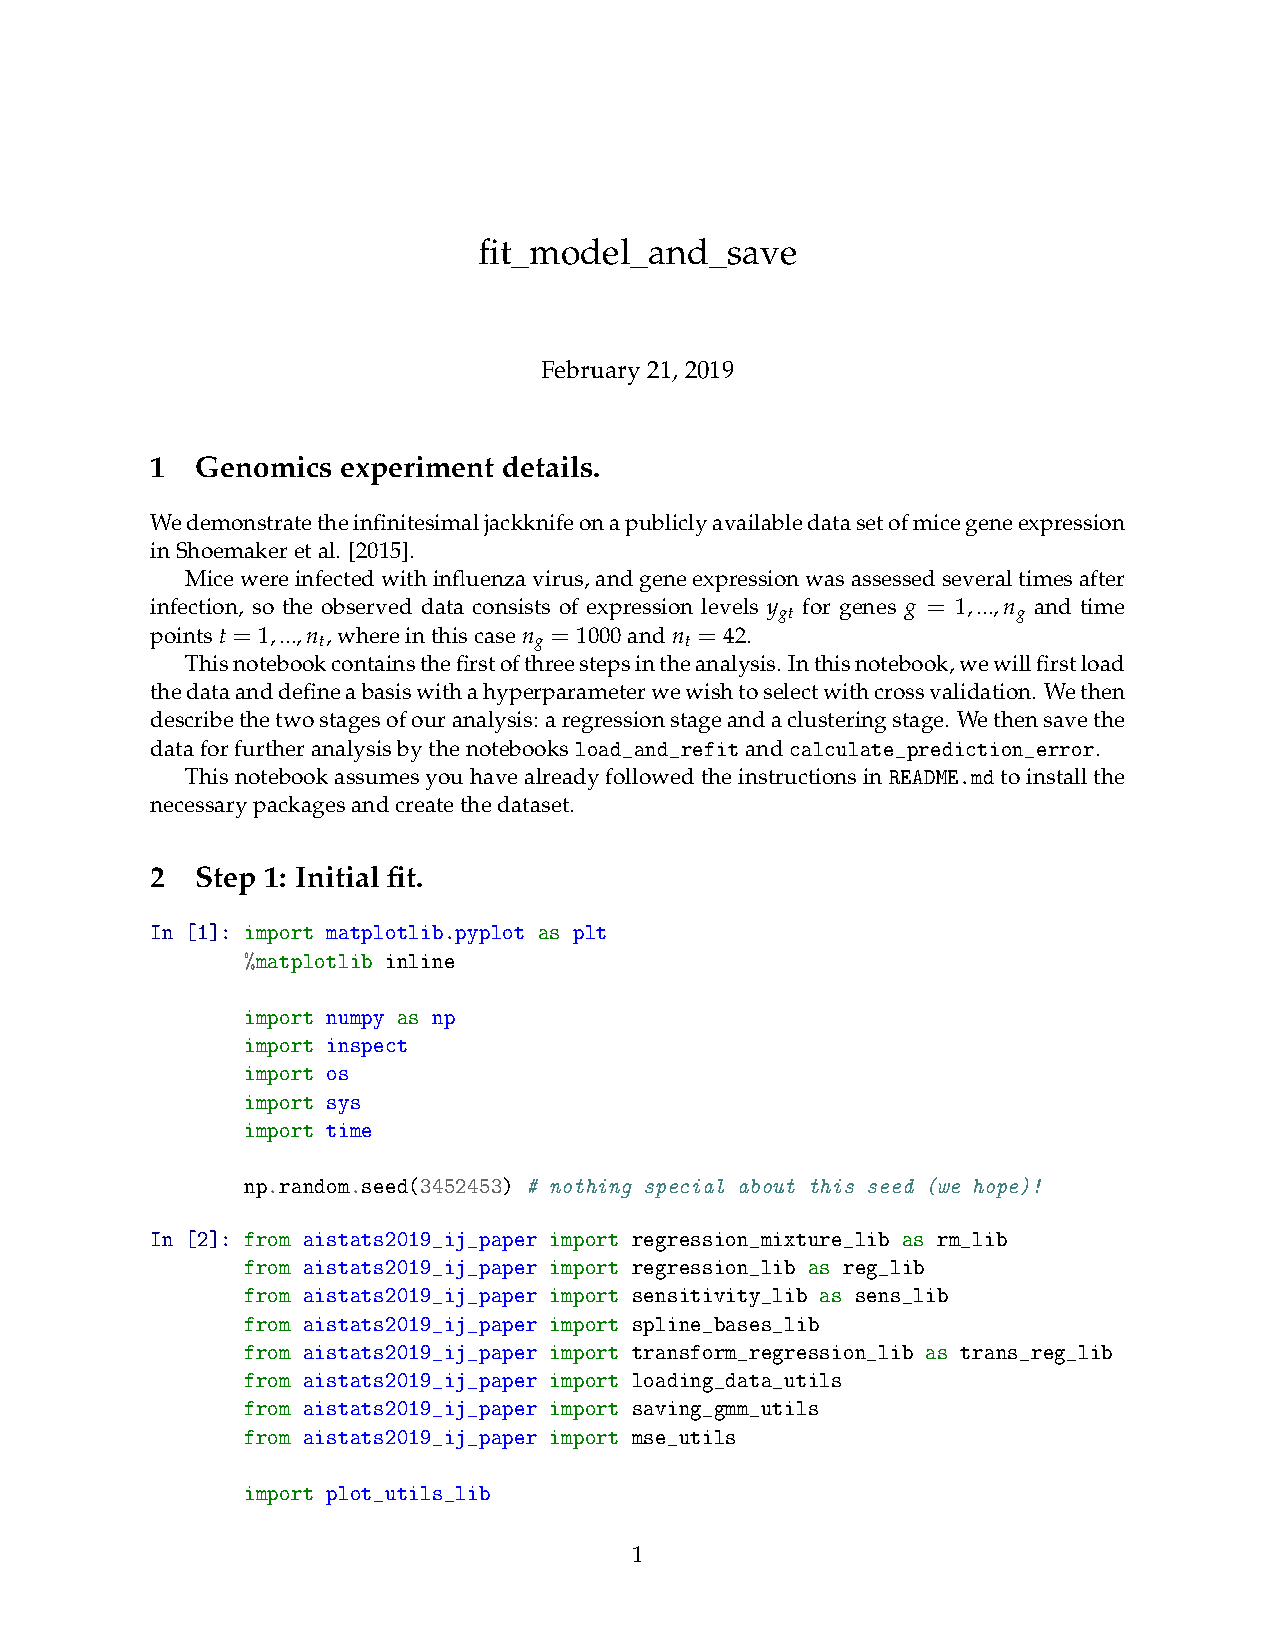
\includepdf[pages=1-, scale=0.8, pagecommand={}]{appendix_pdfs/fit_model_and_save.pdf}
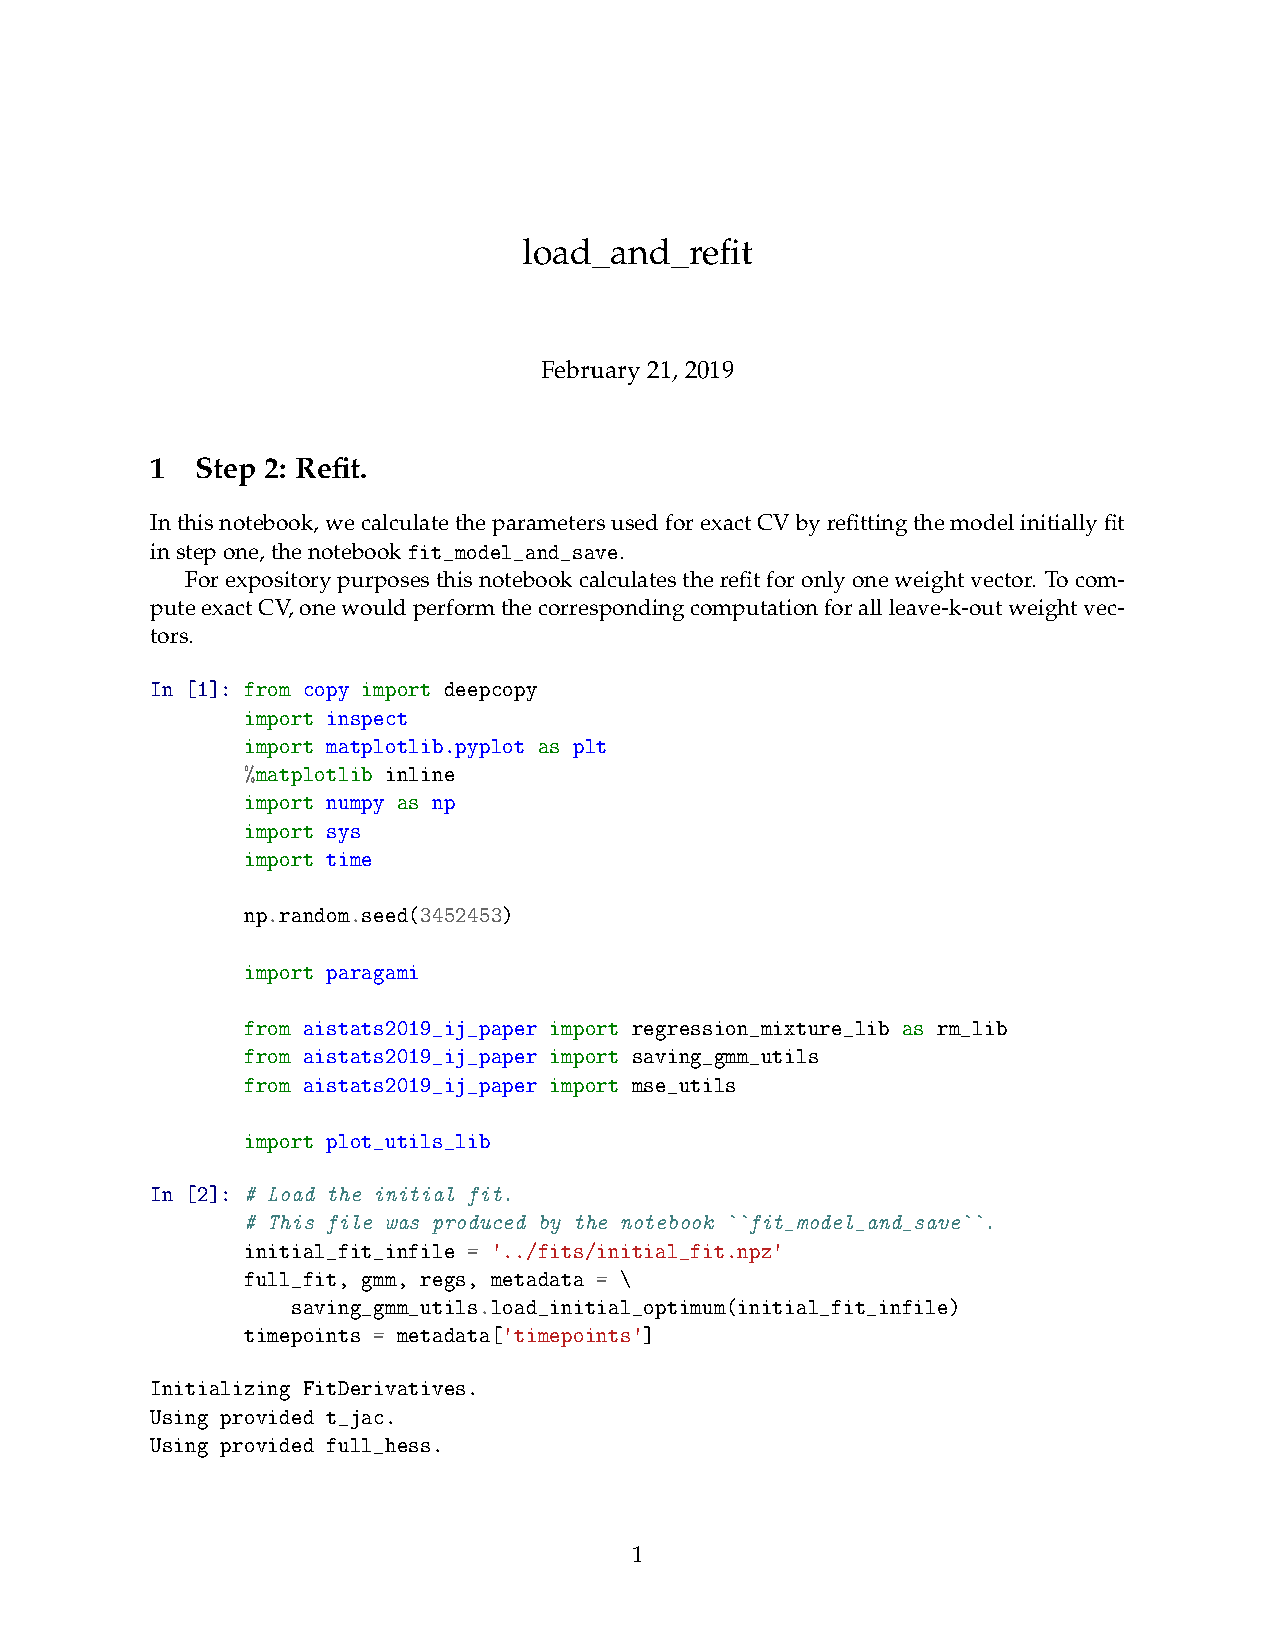
\includepdf[pages=1-, scale=0.8, pagecommand={}]{appendix_pdfs/load_and_refit.pdf}
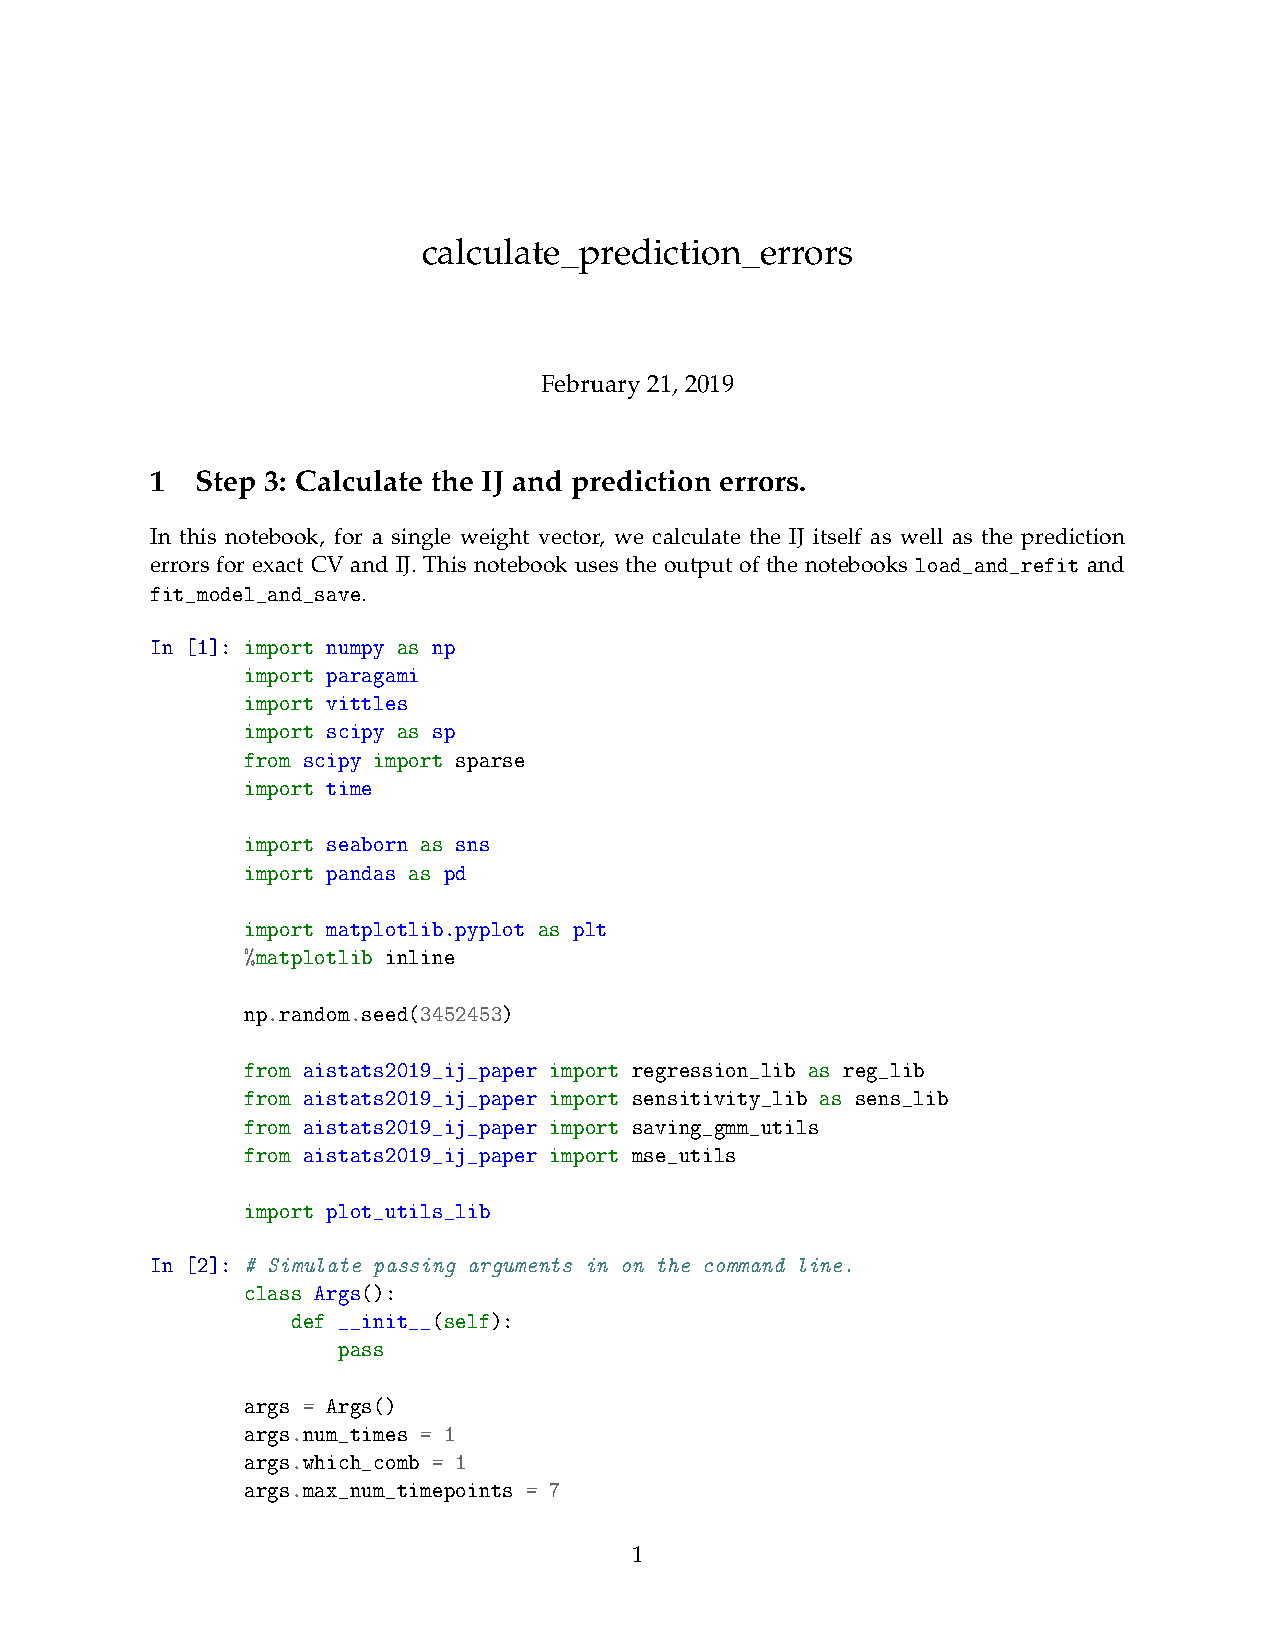
\includepdf[pages=1-, scale=0.8, pagecommand={}]{appendix_pdfs/calculate_prediction_errors.pdf}
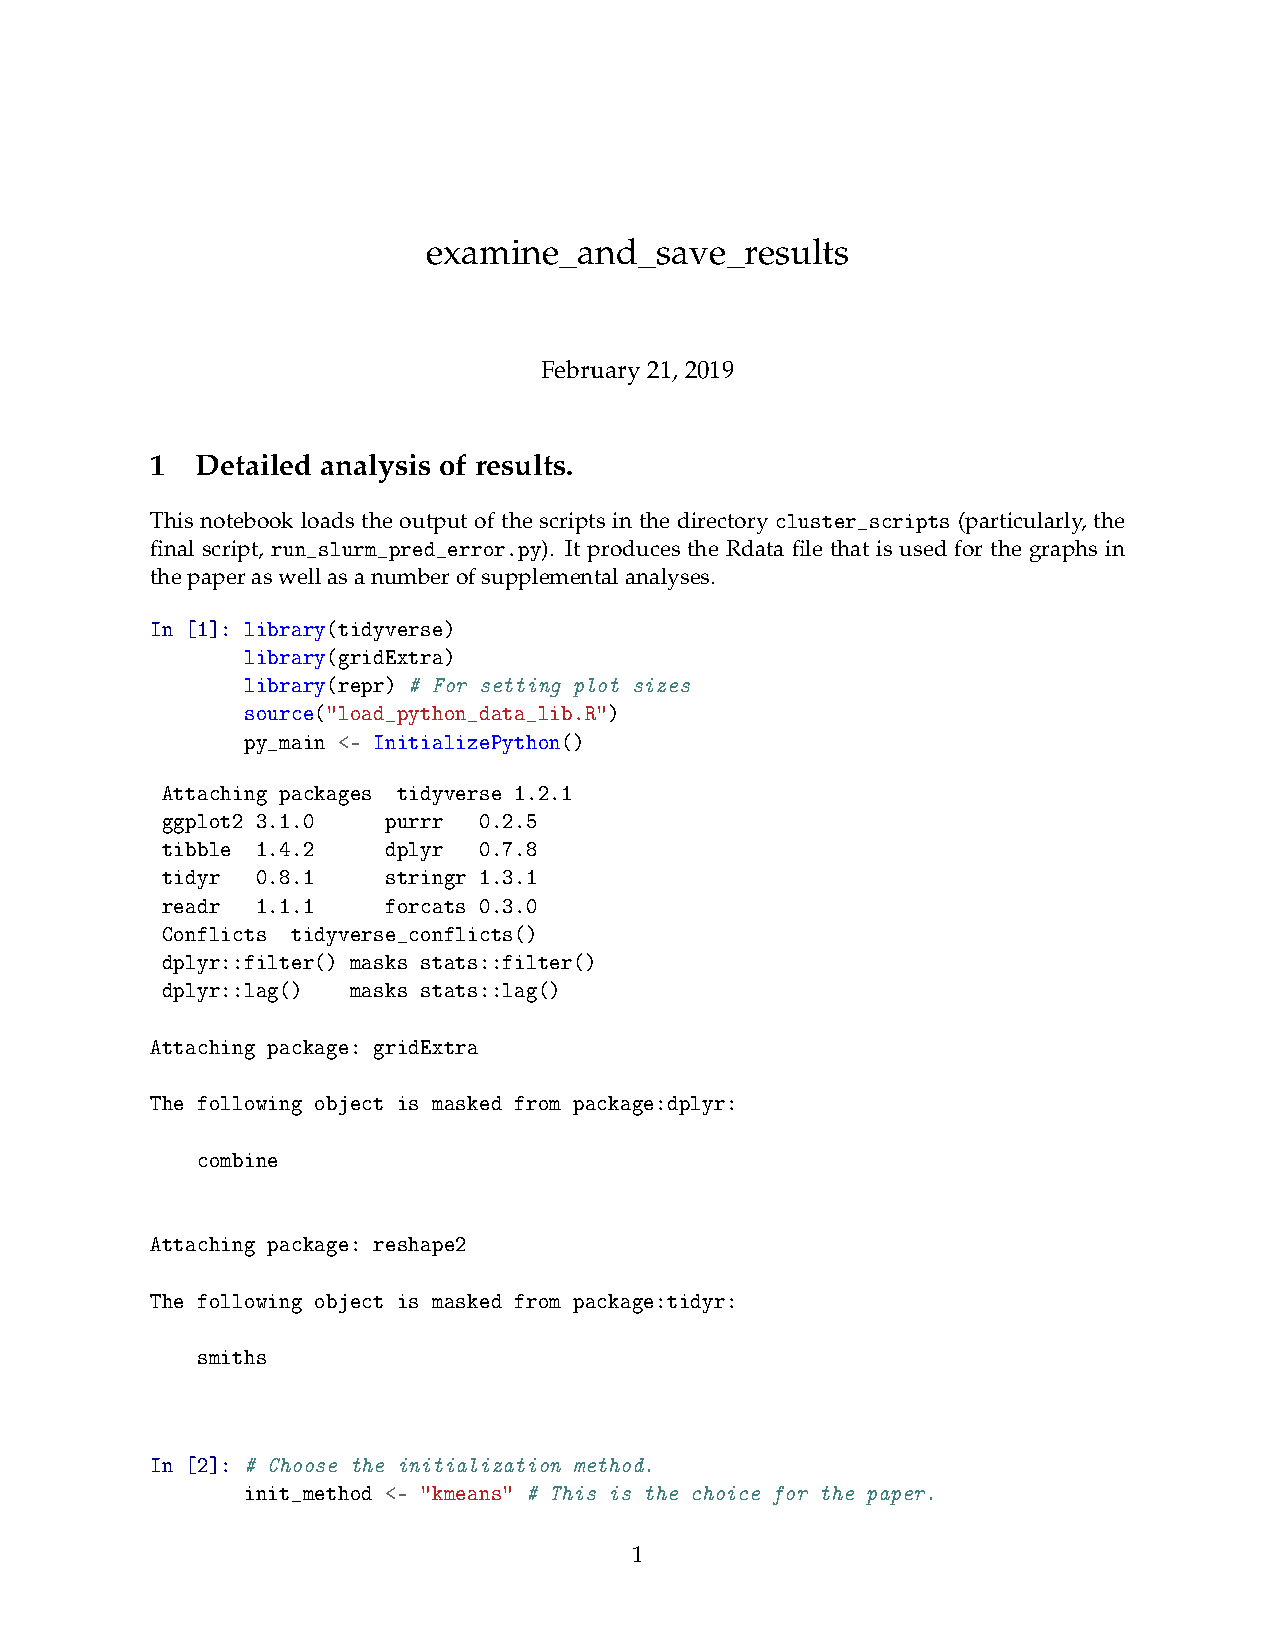
\includepdf[pages=1-, scale=0.8, pagecommand={}]{appendix_pdfs/examine_and_save_results.pdf}

\end{document}
